\documentclass[11pt, letterpaper]{article}

% Fonts and Encoding
\usepackage[utf8]{inputenc}
\usepackage[T1]{fontenc}
\usepackage{lmodern} % High-quality Latin Modern vector font

% Math and Symbols
\usepackage{amsmath, amssymb, amsthm, amsfonts, mathrsfs, mathtools}

% Layout and Geometry
\usepackage{geometry}
\geometry{letterpaper, margin=1in}
\setlength{\parindent}{0pt}
\setlength{\parskip}{0.6em}

% Formatting and Graphics
\usepackage{graphicx, xcolor, enumitem, booktabs, array, tabularx}

% TikZ for Illustrations
\usepackage{tikz}
\usetikzlibrary{arrows.meta, positioning, shapes.geometric, calc, backgrounds, matrix}

% Clickable Links and TOC
\usepackage{hyperref}
\hypersetup{
    colorlinks=true,
    linkcolor=blue,
    filecolor=magenta,      
    urlcolor=cyan,
    pdftitle={Advanced Mathematics Topic},
}

% Theorem Environments
\newtheorem{theorem}{Theorem}[section]
\newtheorem{lemma}[theorem]{Lemma}
\newtheorem{proposition}[theorem]{Proposition}
\newtheorem{corollary}[theorem]{Corollary}
\theoremstyle{definition}
\newtheorem{definition}{Definition}[section]
\newtheorem{axiom}{Axiom}[section]
\newtheorem{example}{Example}[section]
\theoremstyle{remark}
\newtheorem{remark}{Remark}[section]

% Custom Commands (Enforced standard notation)
\newcommand{\R}{\mathbb{R}}
\newcommand{\N}{\mathbb{N}}
\newcommand{\Z}{\mathbb{Z}}
\newcommand{\Q}{\mathbb{Q}}
\newcommand{\E}{\mathbb{E}}
\newcommand{\Prob}{\mathbb{P}}
\newcommand{\F}{\mathcal{F}}

\title{\textbf{Finding the Probability Distribution of a Function of Random Variables: Measure-Theoretic Foundations, Analytical Methods, and Quantitative Applications}}
\author{Tashfeen Omran}
\date{\today}

\begin{document}

\maketitle
\tableofcontents
\newpage

% ==============================================================================
% PART 1: COMPREHENSIVE INTRODUCTION, CONTEXT, AND PREREQUISITES
% ==============================================================================
\section{Comprehensive Introduction, Context, and Prerequisites}

\subsection{Core Concepts and Measure-Theoretic Axioms}

In elementary calculus-based probability, a random variable is often informally described as a "variable whose value is determined by the outcome of a random experiment." In advanced abstract mathematics, however, randomness is formalized through measure theory. To rigorously understand how to find the probability distribution of a function of random variables $U = g(Y_1, Y_2, \dots, Y_n)$, we must construct the mathematical machinery from the ground up.

\begin{definition}[Probability Space]
A \textbf{probability space} is a measure-theoretic triple $(\Omega, \F, \Prob)$, where:
\begin{enumerate}[label=(\roman*)]
    \item $\Omega$ is a non-empty set called the \textbf{sample space}, whose elements $\omega \in \Omega$ represent elementary outcomes.
    \item $\F \subseteq \mathcal{P}(\Omega)$ is a \textbf{$\sigma$-algebra} (or $\sigma$-field) of subsets of $\Omega$, called \textbf{events}, satisfying:
    \begin{enumerate}[label=(\alph*)]
        \item $\Omega \in \F$.
        \item Closure under complementation: If $A \in \F$, then $A^c = \Omega \setminus A \in \F$.
        \item Closure under countable unions: If $\{A_i\}_{i=1}^\infty \subset \F$, then $\bigcup_{i=1}^\infty A_i \in \F$.
    \end{enumerate}
    \item $\Prob: \F \to [0, 1]$ is a \textbf{probability measure} satisfying Kolmogorov's Axioms:
    \begin{enumerate}[label=(\alph*)]
        \item Non-negativity: $\Prob(A) \ge 0$ for all $A \in \F$.
        \item Normalization: $\Prob(\Omega) = 1$.
        \item Countable Additivity ($\sigma$-additivity): For any countable sequence of pairwise disjoint events $\{A_i\}_{i=1}^\infty \subset \F$ (i.e., $A_i \cap A_j = \emptyset$ for $i \neq j$), we have
        \[
            \Prob\left(\bigcup_{i=1}^\infty A_i\right) = \sum_{i=1}^\infty \Prob(A_i).
        \]
    \end{enumerate}
\end{enumerate}
\end{definition}

\begin{definition}[Random Variable and Random Vector]
Let $(\Omega, \F, \Prob)$ be a probability space and let $(\R^n, \mathcal{B}(\R^n))$ be the $n$-dimensional Euclidean space equipped with the \textbf{Borel $\sigma$-algebra} $\mathcal{B}(\R^n)$ (the smallest $\sigma$-algebra containing all open subsets of $\R^n$). A mapping $\mathbf{Y} = (Y_1, Y_2, \dots, Y_n): \Omega \to \R^n$ is an $n$-dimensional \textbf{random vector} (or a collection of $n$ random variables) if it is $(\F, \mathcal{B}(\R^n))$-measurable; that is, for every Borel set $B \in \mathcal{B}(\R^n)$, its pre-image lies in $\F$:
\[
    \mathbf{Y}^{-1}(B) \coloneqq \{\omega \in \Omega : (Y_1(\omega), Y_2(\omega), \dots, Y_n(\omega)) \in B\} \in \F.
\]
\end{definition}

\begin{definition}[Pushforward Measure / Probability Distribution]
Given a random vector $\mathbf{Y}: \Omega \to \R^n$, the \textbf{induced probability distribution} (or \textbf{pushforward measure} $\Prob_{\mathbf{Y}} = \mathbf{Y}_\# \Prob$) is the probability measure on $(\R^n, \mathcal{B}(\R^n))$ defined for all $B \in \mathcal{B}(\R^n)$ by
\[
    \Prob_{\mathbf{Y}}(B) \coloneqq \Prob(\mathbf{Y}^{-1}(B)) = \Prob(\{\omega \in \Omega : \mathbf{Y}(\omega) \in B\}).
\]
If $\Prob_{\mathbf{Y}}$ is absolutely continuous with respect to the $n$-dimensional Lebesgue measure $\lambda_n$ on $\R^n$ (denoted $\Prob_{\mathbf{Y}} \ll \lambda_n$), then by the \textbf{Radon-Nikodym Theorem}, there exists a non-negative Borel-measurable function $f_{\mathbf{Y}}: \R^n \to [0, \infty)$, called the \textbf{joint probability density function (PDF)}, such that for all $B \in \mathcal{B}(\R^n)$:
\[
    \Prob_{\mathbf{Y}}(B) = \int_B f_{\mathbf{Y}}(y_1, y_2, \dots, y_n) \, d\lambda_n(y_1, \dots, y_n).
\]
\end{definition}

\begin{definition}[Random Sample and Statistical Independence]
Random variables $Y_1, Y_2, \dots, Y_n$ are \textbf{mutually independent} if the joint pushforward measure $\Prob_{\mathbf{Y}}$ is the product measure of the marginal pushforward measures:
\[
    \Prob_{\mathbf{Y}} = \bigotimes_{i=1}^n \Prob_{Y_i}.
\]
Equivalently, for all Borel sets $B_1, \dots, B_n \in \mathcal{B}(\R)$, $\Prob(Y_1 \in B_1, \dots, Y_n \in B_n) = \prod_{i=1}^n \Prob(Y_i \in B_i)$. When $Y_1, \dots, Y_n$ are mutually independent and share an identical marginal distribution $\Prob_Y$ (with common PMF $p(y)$ in the discrete case or common PDF $f(y)$ in the continuous case), the collection $(Y_1, \dots, Y_n)$ is called a \textbf{random sample of size $n$} (or i.i.d.\ sample), and its joint density/mass function factors completely:
\[
    p(y_1, y_2, \dots, y_n) = \prod_{i=1}^n p(y_i), \qquad f(y_1, y_2, \dots, y_n) = \prod_{i=1}^n f(y_i).
\]
\end{definition}

\begin{definition}[Function of Random Variables]
Let $\mathbf{Y} = (Y_1, \dots, Y_n): \Omega \to \R^n$ be a random vector and let $g: \R^n \to \R$ be a Borel-measurable function (i.e., $g^{-1}(A) \in \mathcal{B}(\R^n)$ for all $A \in \mathcal{B}(\R)$). The composition
\[
    U \coloneqq g \circ \mathbf{Y} = g(Y_1, Y_2, \dots, Y_n): \Omega \to \R
\]
defined pointwise by $U(\omega) = g(Y_1(\omega), \dots, Y_n(\omega))$ is a new valid random variable on $(\Omega, \F, \Prob)$.
\end{definition}

\subsection{Intuition and Set-Theoretic Foundations}

Why does applying a deterministic function $g: \R^n \to \R$ to random variables $Y_1, \dots, Y_n$ produce another legitimate random variable $U$, and how does probability mass flow from the original space to the transformed space?

The secret lies in the functorial behavior of \textbf{set-theoretic pre-images}. For any subset $A \in \mathcal{B}(\R)$ of target values for $U$, the set of elementary outcomes $\omega \in \Omega$ for which $U(\omega) \in A$ is given by the composition of pre-images:
\[
    U^{-1}(A) = (g \circ \mathbf{Y})^{-1}(A) = \mathbf{Y}^{-1}\big(g^{-1}(A)\big).
\]
Because $g$ is Borel-measurable, the pre-image $R_A \coloneqq g^{-1}(A) = \{(y_1, \dots, y_n) \in \R^n : g(y_1, \dots, y_n) \in A\}$ is guaranteed to be a Borel set in $\mathcal{B}(\R^n)$. Furthermore, because $\mathbf{Y}$ is an $\F$-measurable random vector, the pre-image $\mathbf{Y}^{-1}(R_A)$ is guaranteed to be a measurable event in $\F$. Thus, the probability measure $\Prob$ can legally evaluate this event:
\[
    \Prob_U(A) = \Prob(U \in A) = \Prob\big(\mathbf{Y} \in g^{-1}(A)\big) = \Prob_{\mathbf{Y}}\big(g^{-1}(A)\big) = \idotsint_{g^{-1}(A)} f_{\mathbf{Y}}(y_1, \dots, y_n) \, dy_1 \cdots dy_n.
\]
Intuitively, we never need to return to the abstract sample space $\Omega$. The joint density $f_{\mathbf{Y}}(y_1, \dots, y_n)$ acts as a continuous distribution of "mass" over $\R^n$. The function $g: \R^n \to \R$ slices $\R^n$ into level sets (fibers) $g^{-1}(\{u\})$. To find the cumulative probability $F_U(u) = \Prob(U \le u)$, we simply gather all points $(y_1, \dots, y_n) \in \R^n$ that get mapped by $g$ to a number less than or equal to $u$, and integrate the density $f_{\mathbf{Y}}$ over that $n$-dimensional region. When $g$ stretches or compresses space, the local density of probability mass must scale inversely to the volumetric stretching factor (the Jacobian determinant) so that total probability mass is conserved.

\subsection{Historical Context and Motivation}

The mathematical necessity of finding the probability distribution of a function of random variables originated in the late 18th and early 19th centuries with Pierre-Simon Laplace and Carl Friedrich Gauss in the study of celestial mechanics and geodesy. Astronomers collected noisy measurements $Y_1, Y_2, \dots, Y_n$ of planetary orbits and sought to estimate the true unknown parameter $\mu$ using the arithmetic mean $\bar{Y} = \frac{1}{n}\sum_{i=1}^n Y_i$. Assessing the reliability of $\bar{Y}$ required determining the exact probability distribution of the estimation error $|\bar{Y} - \mu|$ as a function of the $n$ individual measurement errors. Laplace developed early characteristic functions (generating functions) to handle sums of random variables, culminating in the earliest versions of the Central Limit Theorem.

However, a profound foundational crisis emerged in 1889 with Joseph Bertrand's publication of \textbf{Bertrand's Paradox}. Bertrand demonstrated that if one asks for the probability that a "random chord" of a unit circle has length greater than $\sqrt{3}$, three different geometric parameterizations (random midpoint, random polar angle, random radial distance) yield three distinct probabilities: $\frac{1}{4}$, $\frac{1}{3}$, and $\frac{1}{2}$. The paradox exposed a fatal flaw in classical probability: non-linear transformations of continuous variables alter probability densities via Jacobian scaling factors, so "uniformity" is not invariant under non-linear coordinate transformations. This crisis directly motivated Émile Borel, Henri Lebesgue, and ultimately Andrei Nikolaevich Kolmogorov (in his 1933 monograph \textit{Grundbegriffe der Wahrscheinlichkeitsrechnung}) to axiomatize probability via measure theory, establishing that a random variable is a measurable function on a fixed probability space and that transformations of random variables are governed rigorously by pushforward measures and Radon-Nikodym derivatives.

\subsection{Key Theorems, Lemmas, and Formulas}

\begin{theorem}[Preservation of Measurability under Composition]
\label{thm:measurability}
Let $(\Omega, \F)$ be a measurable space, $\mathbf{Y}: \Omega \to \R^n$ be an $(\F, \mathcal{B}(\R^n))$-measurable random vector, and $g: \R^n \to \R^m$ be a $(\mathcal{B}(\R^n), \mathcal{B}(\R^m))$-measurable function. Then the composite function $\mathbf{U} = g \circ \mathbf{Y}: \Omega \to \R^m$ is an $(\F, \mathcal{B}(\R^m))$-measurable random vector.
\end{theorem}

\begin{theorem}[Method 1: The Method of Distribution Functions (CDF Method)]
\label{thm:cdf_method}
Let $\mathbf{Y} = (Y_1, \dots, Y_n)$ be a continuous random vector with joint PDF $f_{\mathbf{Y}}(y_1, \dots, y_n)$ and let $U = g(Y_1, \dots, Y_n)$ be a real-valued Borel-measurable function. The cumulative distribution function (CDF) of $U$ is given for all $u \in \R$ by
\[
    F_U(u) \coloneqq \Prob(U \le u) = \idotsint_{R_u} f_{\mathbf{Y}}(y_1, \dots, y_n) \, dy_1 \cdots dy_n,
\]
where $R_u = \{(y_1, \dots, y_n) \in \R^n : g(y_1, \dots, y_n) \le u\}$. If $F_U(u)$ is absolutely continuous, the probability density function $f_U(u)$ of $U$ is obtained by differentiating $F_U(u)$ with respect to $u$ at all points of differentiability (almost everywhere with respect to Lebesgue measure):
\[
    f_U(u) = \frac{d}{du} F_U(u).
\]
\end{theorem}

\begin{theorem}[Method 2: The Method of Transformations (Univariate and Bivariate)]
\label{thm:transformation_method}
Let $Y$ be a continuous random variable with PDF $f_Y(y)$ supported on an open interval $\mathcal{S}_Y \subseteq \R$. Let $U = h(Y)$, where $h: \mathcal{S}_Y \to \mathcal{S}_U$ is a strictly monotonic (either strictly increasing or strictly decreasing) continuously differentiable bijection ($C^1$-diffeomorphism) with inverse $y = h^{-1}(u)$ and non-vanishing derivative $h'(y) \neq 0$ for all $y \in \mathcal{S}_Y$. Then the PDF of $U$ is given by:
\[
    f_U(u) = \begin{cases}
        \displaystyle f_Y\big(h^{-1}(u)\big) \left| \frac{d}{du} h^{-1}(u) \right|, & u \in \mathcal{S}_U, \\[8pt]
        0, & \text{elsewhere.}
    \end{cases}
\]
In the bivariate setting, if $(Y_1, Y_2)$ has joint PDF $f_{Y_1, Y_2}(y_1, y_2)$ and $U = h(Y_1, Y_2)$ is strictly monotonic in $y_2$ for each fixed $y_1$ with inverse $y_2 = h_1^{-1}(y_1, u)$, then the joint PDF of $(Y_1, U)$ is $f_{Y_1, U}(y_1, u) = f_{Y_1, Y_2}(y_1, h_1^{-1}(y_1, u)) \left|\frac{\partial}{\partial u} h_1^{-1}(y_1, u)\right|$, and the marginal PDF of $U$ is obtained by integrating over $y_1$:
\[
    f_U(u) = \int_{-\infty}^{\infty} f_{Y_1, Y_2}\big(y_1, h_1^{-1}(y_1, u)\big) \left| \frac{\partial}{\partial u} h_1^{-1}(y_1, u) \right| dy_1.
\]
\end{theorem}

\begin{theorem}[Method 3: The Method of Moment-Generating Functions \& Uniqueness (Theorem 6.1)]
\label{thm:mgf_uniqueness}
Let $U$ be a random variable. Its \textbf{moment-generating function (MGF)} is defined as $m_U(t) \coloneqq \E[e^{tU}]$, provided the expectation exists for $t \in (-t_0, t_0)$ for some $t_0 > 0$. 
\begin{enumerate}[label=(\roman*)]
    \item \textbf{Change of Variables (LOTUS)}: If $U = g(Y_1, \dots, Y_n)$, then
    \[
        m_U(t) = \E\big[e^{t g(Y_1, \dots, Y_n)}\big] = \idotsint_{\R^n} e^{t g(y_1, \dots, y_n)} f_{\mathbf{Y}}(y_1, \dots, y_n) \, dy_1 \cdots dy_n.
    \]
    \item \textbf{Factorization for Independent Sums}: If $Y_1, \dots, Y_n$ are mutually independent random variables and $U = \sum_{i=1}^n a_i Y_i + b$, then
    \[
        m_U(t) = e^{bt} \prod_{i=1}^n m_{Y_i}(a_i t).
    \]
    \item \textbf{Uniqueness Theorem (Theorem 6.1)}: Let $U$ and $V$ be two random variables with moment-generating functions $m_U(t)$ and $m_V(t)$, respectively. If there exists $\delta > 0$ such that $m_U(t) = m_V(t) < \infty$ for all $t \in (-\delta, \delta)$, then $U$ and $V$ have identical probability distributions (i.e., $F_U(u) = F_V(u)$ for all $u \in \R$).
\end{enumerate}
\end{theorem}

\begin{theorem}[Method 4: Multivariate Jacobian Transformation Theorem]
\label{thm:jacobian}
Let $\mathbf{Y} = (Y_1, \dots, Y_n)$ have joint PDF $f_{\mathbf{Y}}(\mathbf{y})$ supported on an open set $\mathcal{S}_{\mathbf{Y}} \subseteq \R^n$. Let $\mathbf{h}: \mathcal{S}_{\mathbf{Y}} \to \mathcal{S}_{\mathbf{U}} \subseteq \R^n$ be a $C^1$-diffeomorphism defining $\mathbf{U} = \mathbf{h}(\mathbf{Y})$ with inverse $\mathbf{y} = \mathbf{h}^{-1}(\mathbf{u}) = (w_1(\mathbf{u}), \dots, w_n(\mathbf{u}))$. Then the joint PDF of $\mathbf{U}$ is given by
\[
    f_{\mathbf{U}}(u_1, \dots, u_n) = f_{\mathbf{Y}}\big(w_1(\mathbf{u}), \dots, w_n(\mathbf{u})\big) \cdot |\det J(\mathbf{u})| \, \mathbf{1}_{\mathcal{S}_{\mathbf{U}}}(\mathbf{u}),
\]
where $\det J(\mathbf{u}) = \frac{\partial(w_1, \dots, w_n)}{\partial(u_1, \dots, u_n)}$ is the determinant of the $n \times n$ Jacobian matrix of the inverse transformation.
\end{theorem}

\subsection{Prerequisites}

To master the proofs and computations in this document, the reader must command the following foundational skills:
\begin{itemize}
    \item \textbf{Set Theory and Logic}: Manipulating pre-images ($g^{-1}(A \cup B) = g^{-1}(A) \cup g^{-1}(B)$), De Morgan's laws, indicator functions $\mathbf{1}_A(x)$, and $\sigma$-algebra axioms.
    \item \textbf{Real Analysis and Multivariable Calculus}: The Fundamental Theorem of Calculus, Leibniz's Rule for differentiating parameter-dependent integrals, setting up iterated multiple integrals over non-rectangular geometric domains (simplices, cones, parabolic regions), and computing Jacobian determinants.
    \item \textbf{Linear Algebra and Complex Analysis}: Matrix determinants, positive-definite quadratic forms, and elementary properties of analytic continuation and Fourier/Laplace transforms (for the proof of MGF uniqueness).
\end{itemize}

\newpage
% ==============================================================================
% PART 2: DETAILED HOMEWORK SOLUTIONS (RIGOROUS PROOFS & COMPUTATIONS)
% ==============================================================================
\section{Detailed Homework Solutions (Rigorous Proofs and Computations)}

In this section, we state and rigorously solve every theoretical proposition, estimation problem, and applied example presented in the provided text (Sections 6.2 and 6.3, pages 297--298).

% ------------------------------------------------------------------------------
% PROBLEM 1
% ------------------------------------------------------------------------------
\subsection{Problem 1: Estimation Error and Joint Distribution of a Random Sample (Page 297)}

\textbf{Original Problem Statement (Extracted from Page 297):}
\begin{quote}
\textit{``Consider the sample mean $\bar{Y} = (1/n)\sum_{i=1}^n Y_i$ as an estimate for $\mu$. How good is this estimate? The answer depends upon the behavior of the random variables $Y_1, Y_2, \dots, Y_n$ and their effect on the distribution of $\bar{Y} = (1/n)\sum_{i=1}^n Y_i$. A measure of the goodness of an estimate is the error of estimation, the difference between the estimate and the parameter estimated (for our example, the difference between $\bar{y}$ and $\mu$). Because $Y_1, Y_2, \dots, Y_n$ are random variables, in repeated sampling $\bar{Y}$ is also a random variable (and a function of the $n$ variables $Y_1, Y_2, \dots, Y_n$). Therefore, we cannot be certain that the error of estimation will be less than a specific value, say, $B$. However, if we can determine the probability distribution of the estimator $\bar{Y}$, this probability distribution can be used to determine the probability that the error of estimation is less than or equal to $B$. ... Thus, in the discrete case, the joint probability function for $Y_1, Y_2, \dots, Y_n$, all sampled from the same population, is given by $p(y_1, y_2, \dots, y_n) = p(y_1)p(y_2)\cdots p(y_n)$. In the continuous case, the joint density function is $f(y_1, y_2, \dots, y_n) = f(y_1)f(y_2)\cdots f(y_n)$.''}
\end{quote}

\textbf{Required Tasks:}
\begin{enumerate}[label=(\alph*)]
    \item Prove from first principles of measure theory that if $Y_1, Y_2, \dots, Y_n$ are random variables on $(\Omega, \F, \Prob)$, then the sample mean $\bar{Y} = \frac{1}{n}\sum_{i=1}^n Y_i$ and the error of estimation $E = |\bar{Y} - \mu|$ are valid $(\F, \mathcal{B}(\R))$-measurable random variables.
    \item Prove that if $Y_1, Y_2, \dots, Y_n$ form a random sample (independent and identically distributed) from a population with PMF $p(y)$ (discrete case) or PDF $f(y)$ (continuous case), then their joint PMF/PDF factors as $p(y_1, \dots, y_n) = \prod_{i=1}^n p(y_i)$ and $f(y_1, \dots, y_n) = \prod_{i=1}^n f(y_i)$.
    \item Formulate the exact $n$-dimensional measure-theoretic integral representing the probability that the error of estimation is at most $B > 0$, i.e., $\Prob(|\bar{Y} - \mu| \le B)$. Then, evaluate the distribution of $\bar{Y}$ and $\Prob(|\bar{Y} - \mu| \le B)$ explicitly when $Y_1, \dots, Y_n$ is a random sample from a Normal population $f(y) = \frac{1}{\sqrt{2\pi}\sigma}\exp\left(-\frac{(y-\mu)^2}{2\sigma^2}\right)$.
\end{enumerate}

\hr
\textbf{Rigorous Proof and Solution:}

\subsubsection*{Part (a): Direct Proof of Measurability of $\bar{Y}$ and $|\bar{Y} - \mu|$}
\textbf{Proof Technique:} Direct Proof via Topological Continuity and Borel Measurability Preservation.

\begin{proof}
Let $(\Omega, \F, \Prob)$ be the underlying probability space. By hypothesis, each $Y_i: \Omega \to \R$ ($i = 1, \dots, n$) is an $(\F, \mathcal{B}(\R))$-measurable function.
\begin{enumerate}[label=\textbf{Step \arabic*:}]
    \item \textit{Measurability of the Random Vector $\mathbf{Y}$}: Define the mapping $\mathbf{Y}: \Omega \to \R^n$ by $\mathbf{Y}(\omega) = (Y_1(\omega), \dots, Y_n(\omega))$. Recall that the Borel $\sigma$-algebra on $\R^n$ coincides with the $n$-fold product $\sigma$-algebra: $\mathcal{B}(\R^n) = \bigotimes_{i=1}^n \mathcal{B}(\R)$, which is generated by the family of measurable rectangles $\mathcal{R} = \{B_1 \times B_2 \times \cdots \times B_n : B_i \in \mathcal{B}(\R)\}$. For any generator $B_1 \times \cdots \times B_n \in \mathcal{R}$, the pre-image under $\mathbf{Y}$ is:
    \[
        \mathbf{Y}^{-1}(B_1 \times \cdots \times B_n) = \{\omega \in \Omega : Y_1(\omega) \in B_1 \text{ and } \cdots \text{ and } Y_n(\omega) \in B_n\} = \bigcap_{i=1}^n Y_i^{-1}(B_i).
    \]
    Since each $Y_i$ is measurable, $Y_i^{-1}(B_i) \in \F$ for each $i = 1, \dots, n$. Because a $\sigma$-algebra $\F$ is closed under finite intersections, $\bigcap_{i=1}^n Y_i^{-1}(B_i) \in \F$. Since the pre-images of a generating set of $\mathcal{B}(\R^n)$ lie in $\F$, $\mathbf{Y}$ is $(\F, \mathcal{B}(\R^n))$-measurable.
    
    \item \textit{Continuity and Borel Measurability of the Averaging Map}: Define $g: \R^n \to \R$ by
    \[
        g(y_1, y_2, \dots, y_n) = \frac{1}{n} \sum_{i=1}^n y_i.
    \]
    Since $g$ is a linear combination of coordinate projections, $g$ is continuous with respect to the standard Euclidean topologies on $\R^n$ and $\R$. By definition of continuous functions, for every open set $V \subseteq \R$, $g^{-1}(V)$ is open in $\R^n$, which implies $g^{-1}(V) \in \mathcal{B}(\R^n)$. Since open sets generate $\mathcal{B}(\R)$, $g$ is $(\mathcal{B}(\R^n), \mathcal{B}(\R))$-measurable.
    
    \item \textit{Composition for $\bar{Y}$}: By Theorem \ref{thm:measurability}, for any $A \in \mathcal{B}(\R)$,
    \[
        \bar{Y}^{-1}(A) = (g \circ \mathbf{Y})^{-1}(A) = \mathbf{Y}^{-1}\big(g^{-1}(A)\big) \in \F.
    \]
    Hence, $\bar{Y} = \frac{1}{n}\sum_{i=1}^n Y_i$ is a valid random variable on $(\Omega, \F, \Prob)$.
    
    \item \textit{Measurability of the Error of Estimation $E = |\bar{Y} - \mu|$}: Define $h: \R \to \R$ by $h(x) = |x - \mu|$. By the reverse triangle inequality, $|h(x) - h(z)| = \big||x - \mu| - |z - \mu|\big| \le |x - z|$, so $h$ is Lipschitz continuous with Lipschitz constant $L = 1$, and therefore Borel-measurable. Consequently, the composition $E = h \circ \bar{Y} = |\bar{Y} - \mu|$ is $(\F, \mathcal{B}(\R))$-measurable and thus a valid random variable.
\end{enumerate}
\end{proof}

\subsubsection*{Part (b): Direct Proof of Joint PMF and Joint PDF Factorization}
\textbf{Proof Technique:} Direct Proof using Measure-Theoretic Independence and Fubini-Tonelli Theorem.

\begin{proof}
Let $Y_1, Y_2, \dots, Y_n$ be mutually independent and identically distributed random variables on $(\Omega, \F, \Prob)$.
\begin{enumerate}[label=\textbf{Case \arabic*:}]
    \item \textbf{Discrete Case}: Suppose each $Y_i$ takes values in a countable support $\mathcal{S} \subseteq \R$ with common marginal probability mass function $p(y) = \Prob(Y_i = y)$. By the definition of the joint probability mass function at any point $(y_1, y_2, \dots, y_n) \in \mathcal{S}^n$:
    \[
        p(y_1, y_2, \dots, y_n) \coloneqq \Prob(Y_1 = y_1, Y_2 = y_2, \dots, Y_n = y_n) = \Prob\left(\bigcap_{i=1}^n Y_i^{-1}(\{y_i\})\right).
    \]
    Since every singleton $\{y_i\} \in \mathcal{B}(\R)$, mutual independence of $Y_1, \dots, Y_n$ directly implies:
    \[
        \Prob\left(\bigcap_{i=1}^n Y_i^{-1}(\{y_i\})\right) = \prod_{i=1}^n \Prob\big(Y_i^{-1}(\{y_i\})\big) = \prod_{i=1}^n \Prob(Y_i = y_i) = p(y_1)p(y_2)\cdots p(y_n).
    \]
    
    \item \textbf{Continuous Case}: Suppose each $Y_i$ is absolutely continuous with respect to the 1-dimensional Lebesgue measure $\lambda_1$ with common Radon-Nikodym derivative (PDF) $f(y)$, so that $\Prob(Y_i \in B_i) = \int_{B_i} f(y_i) \, d\lambda_1(y_i)$ for every $B_i \in \mathcal{B}(\R)$. Consider any measurable rectangle $R = B_1 \times B_2 \times \cdots \times B_n \in \mathcal{B}(\R^n)$. By mutual independence:
    \[
        \Prob_{\mathbf{Y}}(R) = \Prob(Y_1 \in B_1, \dots, Y_n \in B_n) = \prod_{i=1}^n \Prob(Y_i \in B_i) = \prod_{i=1}^n \left( \int_{B_i} f(y_i) \, dy_i \right).
    \]
    Since $f(y_i) \ge 0$ is non-negative and measurable for each $i$, Tonelli's Theorem allows us to rewrite the product of $n$ one-dimensional Lebesgue integrals as an $n$-dimensional iterated integral over the product space $R = B_1 \times \cdots \times B_n$:
    \[
        \Prob_{\mathbf{Y}}(R) = \int_{B_1} \int_{B_2} \cdots \int_{B_n} f(y_1)f(y_2)\cdots f(y_n) \, dy_n \cdots dy_2 \, dy_1 = \idotsint_R \left(\prod_{i=1}^n f(y_i)\right) d\lambda_n(\mathbf{y}).
    \]
    By Carathéodory's Extension Theorem ($\pi$-$\lambda$ Dynkin System Theorem), because the set of measurable rectangles is a $\pi$-system generating $\mathcal{B}(\R^n)$, the equality $\Prob_{\mathbf{Y}}(B) = \idotsint_B \left(\prod_{i=1}^n f(y_i)\right) d\lambda_n(\mathbf{y})$ holds for all $B \in \mathcal{B}(\R^n)$. By uniqueness of the Radon-Nikodym derivative up to sets of Lebesgue measure zero, the joint density is:
    \[
        f(y_1, y_2, \dots, y_n) = f(y_1)f(y_2)\cdots f(y_n).
    \]
\end{enumerate}
\end{proof}

\subsubsection*{Part (c): Formulation and Explicit Evaluation of the Estimation Error Probability}
Let $B > 0$ be the specified error bound. The event that the error of estimation is at most $B$ is:
\[
    A_B = \{\omega \in \Omega : |\bar{Y}(\omega) - \mu| \le B\} = \left\{\omega \in \Omega : \mu - B \le \frac{1}{n}\sum_{i=1}^n Y_i(\omega) \le \mu + B\right\}.
\]
In $\R^n$, this defines the $n$-dimensional slab region (bounded between two parallel hyperplanes):
\[
    \mathcal{D}_B = \left\{(y_1, \dots, y_n) \in \R^n : n(\mu - B) \le \sum_{i=1}^n y_i \le n(\mu + B)\right\}.
\]
Therefore, using the joint density of a random sample, the exact probability is:
\[
    \Prob(|\bar{Y} - \mu| \le B) = \idotsint_{\mathcal{D}_B} \left(\prod_{i=1}^n f(y_i)\right) dy_1 \, dy_2 \cdots dy_n.
\]
Rather than integrating directly over the $n$-dimensional hyperplane slab $\mathcal{D}_B$, we apply **Method 3 (The Method of Moment-Generating Functions)** from Section 6.2 to find the exact distribution of $\bar{Y}$ when $Y_i \stackrel{\text{i.i.d.}}{\sim} \mathcal{N}(\mu, \sigma^2)$:
\begin{enumerate}[label=\textbf{Step \arabic*:}]
    \item The MGF of a single Normal random variable $Y_i \sim \mathcal{N}(\mu, \sigma^2)$ is known to be:
    \[
        m_{Y_i}(t) = \E[e^{t Y_i}] = \exp\left(\mu t + \frac{1}{2}\sigma^2 t^2\right), \quad \forall t \in \R.
    \]
    \item Express $\bar{Y} = \sum_{i=1}^n \frac{1}{n} Y_i$. By definition of the MGF and mutual independence of $Y_1, \dots, Y_n$:
    \begin{align*}
        m_{\bar{Y}}(t) &= \E\left[e^{t \bar{Y}}\right] = \E\left[\exp\left(\sum_{i=1}^n \frac{t}{n} Y_i\right)\right] = \E\left[\prod_{i=1}^n e^{(t/n) Y_i}\right] \\
        &= \prod_{i=1}^n \E\left[e^{(t/n) Y_i}\right] \quad \text{(by mutual independence)} \\
        &= \prod_{i=1}^n m_{Y_i}\left(\frac{t}{n}\right) = \prod_{i=1}^n \exp\left(\mu\left(\frac{t}{n}\right) + \frac{1}{2}\sigma^2\left(\frac{t}{n}\right)^2\right) \\
        &= \exp\left(\sum_{i=1}^n \frac{\mu t}{n} + \sum_{i=1}^n \frac{\sigma^2 t^2}{2n^2}\right) = \exp\left(\mu t + \frac{1}{2}\left(\frac{\sigma^2}{n}\right) t^2\right).
    \end{align*}
    \item We recognize $m_{\bar{Y}}(t) = \exp\left(\mu t + \frac{1}{2}\left(\frac{\sigma}{\sqrt{n}}\right)^2 t^2\right)$ as the exact MGF of a Normal distribution with mean $\mu$ and variance $\frac{\sigma^2}{n}$. By **Theorem 6.1 (Uniqueness of MGFs)**, $\bar{Y} \sim \mathcal{N}\left(\mu, \frac{\sigma^2}{n}\right)$, with PDF:
    \[
        f_{\bar{Y}}(\bar{y}) = \frac{\sqrt{n}}{\sqrt{2\pi}\sigma} \exp\left(-\frac{n(\bar{y} - \mu)^2}{2\sigma^2}\right), \quad \bar{y} \in \R.
    \]
    \item Consequently, the probability that the error of estimation is at most $B$ reduces from an $n$-dimensional integral to a $1$-dimensional Gaussian integral:
    \[
        \Prob(|\bar{Y} - \mu| \le B) = \int_{\mu - B}^{\mu + B} \frac{\sqrt{n}}{\sqrt{2\pi}\sigma} \exp\left(-\frac{n(\bar{y} - \mu)^2}{2\sigma^2}\right) d\bar{y}.
    \]
    Applying the univariate transformation $z = \frac{\sqrt{n}(\bar{y} - \mu)}{\sigma}$ (so $dz = \frac{\sqrt{n}}{\sigma} d\bar{y}$), we obtain:
    \[
        \Prob(|\bar{Y} - \mu| \le B) = \int_{-\frac{B\sqrt{n}}{\sigma}}^{\frac{B\sqrt{n}}{\sigma}} \frac{1}{\sqrt{2\pi}} e^{-z^2/2} \, dz = 2\Phi\left(\frac{B\sqrt{n}}{\sigma}\right) - 1,
    \]
    where $\Phi(z) = \int_{-\infty}^z \frac{1}{\sqrt{2\pi}} e^{-w^2/2} \, dw$ is the standard normal CDF. Notice that as $n \to \infty$, $\frac{B\sqrt{n}}{\sigma} \to \infty$, so $\Prob(|\bar{Y} - \mu| \le B) \to 2(1) - 1 = 1$, proving consistency of $\bar{Y}$ (Weak Law of Large Numbers). \hfill $\blacksquare$
\end{enumerate}

% ------------------------------------------------------------------------------
% PROBLEM 2
% ------------------------------------------------------------------------------
\subsection{Problem 2: Rigorous Proofs of the Three Methods in Section 6.2 (Page 298)}

\textbf{Original Problem Statement (Extracted from Page 298):}
\begin{quote}
\textit{``Consider random variables $Y_1, Y_2, \dots, Y_n$ and a function $U(Y_1, Y_2, \dots, Y_n)$, denoted simply as $U$. Then three of the methods for finding the probability distribution of $U$ are as follows:
1. The method of distribution functions: First, find the distribution function for $U$, $F_U(u) = P(U \le u)$... by integrating $f(y_1, y_2, \dots, y_n)$ over the region for which $U \le u$. The density function for $U$ is then obtained by differentiating the distribution function, $F_U(u)$.
2. The method of transformations: If we are given the density function of a random variable $Y$, the method of transformations results in a general expression for the density of $U = h(Y)$ for an increasing or decreasing function $h(y)$. Then if $Y_1$ and $Y_2$ have a bivariate distribution, we can use the univariate result explained earlier to find the joint density of $Y_1$ and $U = h(Y_1, Y_2)$. By integrating over $y_1$, we find the marginal probability density function of $U$.
3. The method of moment-generating functions: This method is based on a uniqueness theorem, Theorem 6.1, which states that, if two random variables have identical moment-generating functions, the two random variables possess the same probability distributions.''}
\end{quote}

\textbf{Required Tasks:}
Provide complete, rigorous mathematical proofs establishing the validity of:
\begin{enumerate}[label=(\alph*)]
    \item Method 1 (The Method of Distribution Functions), verifying that $F_U(u)$ satisfies all axioms of a cumulative distribution function.
    \item Method 2 (The Method of Transformations), proving both the univariate formula $f_U(u) = f_Y(h^{-1}(u)) \left|\frac{d}{du}h^{-1}(u)\right|$ (for both strictly increasing and strictly decreasing $h$) and the bivariate marginalization formula $f_U(u) = \int_{-\infty}^\infty f_{Y_1, Y_2}(y_1, h_1^{-1}(y_1, u)) \left|\frac{\partial}{\partial u}h_1^{-1}(y_1, u)\right| dy_1$.
    \item Method 3 (The Method of Moment-Generating Functions), proving how the existence and equality of MGFs on an open interval $(-\delta, \delta)$ uniquely determines the probability distribution via analytic continuation and Fourier inversion.
\end{enumerate}

\hr
\textbf{Rigorous Proof and Solution:}

\subsubsection*{Part (a): Proof of Method 1 (Method of Distribution Functions)}
\textbf{Proof Technique:} Direct Measure-Theoretic Proof using Continuity of Measure and the Lebesgue Differentiation Theorem.

\begin{proof}
Let $\mathbf{Y} = (Y_1, \dots, Y_n)$ have joint PDF $f_{\mathbf{Y}}(\mathbf{y})$ and let $U = g(\mathbf{Y})$ be Borel-measurable. Define $R_u = \{\mathbf{y} \in \R^n : g(\mathbf{y}) \le u\} = g^{-1}((-\infty, u])$. Since $(-\infty, u] \in \mathcal{B}(\R)$ and $g$ is Borel-measurable, $R_u \in \mathcal{B}(\R^n)$. By definition of the pushforward measure:
\[
    F_U(u) = \Prob(U \le u) = \Prob(\mathbf{Y} \in R_u) = \idotsint_{R_u} f_{\mathbf{Y}}(y_1, \dots, y_n) \, dy_1 \cdots dy_n.
\]
We verify that $F_U(u)$ satisfies the three defining axioms of a Cumulative Distribution Function:
\begin{enumerate}[label=\textbf{Axiom \arabic*:}]
    \item \textit{Monotonicity (Non-decreasing)}: Let $u_1 < u_2$. Then $(-\infty, u_1] \subset (-\infty, u_2]$, which implies $R_{u_1} \subseteq R_{u_2}$ and $R_{u_2} \setminus R_{u_1} = \{\mathbf{y} \in \R^n : u_1 < g(\mathbf{y}) \le u_2\}$. Since $f_{\mathbf{Y}}(\mathbf{y}) \ge 0$ everywhere:
    \[
        F_U(u_2) - F_U(u_1) = \idotsint_{R_{u_2} \setminus R_{u_1}} f_{\mathbf{Y}}(\mathbf{y}) \, d\mathbf{y} \ge 0 \implies F_U(u_1) \le F_U(u_2).
    \]
    \item \textit{Right-Continuity}: Let $\{u_k\}_{k=1}^\infty$ be a monotonically decreasing sequence such that $u_1 > u_2 > \cdots$ and $\lim_{k\to\infty} u_k = u$. Then $R_{u_1} \supseteq R_{u_2} \supseteq \cdots$ is a decreasing sequence of Borel sets with $\bigcap_{k=1}^\infty R_{u_k} = \{\mathbf{y} : g(\mathbf{y}) \le u\} = R_u$. Since $\Prob_{\mathbf{Y}}(\R^n) = 1 < \infty$, by **Continuity of Measure from Above**:
    \[
        \lim_{k \to \infty} F_U(u_k) = \lim_{k \to \infty} \Prob_{\mathbf{Y}}(R_{u_k}) = \Prob_{\mathbf{Y}}\left(\bigcap_{k=1}^\infty R_{u_k}\right) = \Prob_{\mathbf{Y}}(R_u) = F_U(u).
    \]
    \item \textit{Asymptotic Limits at $\pm\infty$}: Let $u_k = -k$ for $k \in \N$. Then $R_{-k}$ is a decreasing sequence of sets with $\bigcap_{k=1}^\infty R_{-k} = \emptyset$ (since $g(\mathbf{y}) \in \R$). By Continuity from Above, $\lim_{u \to -\infty} F_U(u) = \Prob_{\mathbf{Y}}(\emptyset) = 0$. Similarly, let $u_k = k$. Then $R_k$ is an increasing sequence of sets with $\bigcup_{k=1}^\infty R_k = \R^n$. By **Continuity of Measure from Below**, $\lim_{u \to \infty} F_U(u) = \Prob_{\mathbf{Y}}(\R^n) = 1$.
\end{enumerate}
Finally, if $F_U(u)$ is absolutely continuous with respect to Lebesgue measure on $\R$, then by the Fundamental Theorem of Calculus for Lebesgue Integrals (Lebesgue Differentiation Theorem), there exists a density $f_U(u)$ such that $F_U(u) = \int_{-\infty}^u f_U(t) \, dt$, and at every point $u$ where $F_U$ is differentiable:
\[
    \frac{d}{du} F_U(u) = \frac{d}{du} \int_{-\infty}^u f_U(t) \, dt = f_U(u).
\]
\end{proof}

\subsubsection*{Part (b): Proof of Method 2 (Method of Transformations)}
\textbf{Proof Technique:} Direct Proof by Case Analysis on Monotonicity and Application of Leibniz's Integral Rule.

\begin{proof}
Let $Y$ have continuous PDF $f_Y(y)$ on an open interval $\mathcal{S}_Y \subseteq \R$, and let $U = h(Y)$ where $h: \mathcal{S}_Y \to \mathcal{S}_U$ is a $C^1$-diffeomorphism with inverse $w(u) \coloneqq h^{-1}(u)$.

\textbf{Part 1: Univariate Transformation.} We divide into two exhaustive cases based on the sign of $h'(y)$:
\begin{itemize}
    \item \textbf{Case 1: $h$ is strictly increasing ($h'(y) > 0$ on $\mathcal{S}_Y$).} Then the inverse $w(u) = h^{-1}(u)$ is also strictly increasing ($w'(u) > 0$ on $\mathcal{S}_U$). Consequently, for any $u \in \mathcal{S}_U$, the inequality $h(Y) \le u$ is logically equivalent to $Y \le h^{-1}(u)$:
    \[
        \{y \in \mathcal{S}_Y : h(y) \le u\} = \{y \in \mathcal{S}_Y : y \le h^{-1}(u)\}.
    \]
    Applying Method 1 (the CDF Method):
    \[
        F_U(u) = \Prob(U \le u) = \Prob(h(Y) \le u) = \Prob\big(Y \le h^{-1}(u)\big) = \int_{-\infty}^{h^{-1}(u)} f_Y(y) \, dy = F_Y\big(h^{-1}(u)\big).
    \]
    Differentiating both sides with respect to $u$ via the Chain Rule and Fundamental Theorem of Calculus yields:
    \[
        f_U(u) = \frac{d}{du} F_U(u) = \frac{d}{du} \left[ F_Y\big(h^{-1}(u)\big) \right] = f_Y\big(h^{-1}(u)\big) \cdot \frac{d}{du} h^{-1}(u).
    \]
    Since $h^{-1}$ is strictly increasing, $\frac{d}{du}h^{-1}(u) > 0$, so $\frac{d}{du}h^{-1}(u) = \left|\frac{d}{du}h^{-1}(u)\right|$.

    \item \textbf{Case 2: $h$ is strictly decreasing ($h'(y) < 0$ on $\mathcal{S}_Y$).} Then the inverse $w(u) = h^{-1}(u)$ is also strictly decreasing ($w'(u) < 0$ on $\mathcal{S}_U$). Applying $h^{-1}$ to both sides of $h(Y) \le u$ reverses the inequality direction:
    \[
        \{y \in \mathcal{S}_Y : h(y) \le u\} = \{y \in \mathcal{S}_Y : y \ge h^{-1}(u)\}.
    \]
    Therefore, the CDF of $U$ is:
    \[
        F_U(u) = \Prob(U \le u) = \Prob(h(Y) \le u) = \Prob\big(Y \ge h^{-1}(u)\big) = \int_{h^{-1}(u)}^{\infty} f_Y(y) \, dy = 1 - F_Y\big(h^{-1}(u)\big).
    \]
    Differentiating both sides with respect to $u$ via the Chain Rule gives:
    \[
        f_U(u) = \frac{d}{du} F_U(u) = \frac{d}{du}\left[1 - F_Y\big(h^{-1}(u)\big)\right] = -f_Y\big(h^{-1}(u)\big) \cdot \frac{d}{du} h^{-1}(u).
    \]
    Because $h^{-1}$ is strictly decreasing, $\frac{d}{du}h^{-1}(u) < 0$, which means $-\frac{d}{du}h^{-1}(u) = \left|\frac{d}{du}h^{-1}(u)\right| > 0$.
\end{itemize}
Combining Case 1 and Case 2 into a single unified expression yields:
\[
    f_U(u) = f_Y\big(h^{-1}(u)\big) \left| \frac{d}{du} h^{-1}(u) \right|, \quad u \in \mathcal{S}_U.
\]

\textbf{Part 2: Bivariate Extension.} Let $(Y_1, Y_2)$ have joint density $f_{Y_1, Y_2}(y_1, y_2)$ and let $U = h(Y_1, Y_2)$, where for each fixed $y_1$, the mapping $y_2 \mapsto h(y_1, y_2)$ is strictly increasing (the strictly decreasing case is analogous) with partial inverse $y_2 = h_1^{-1}(y_1, u)$. Consider the joint CDF of $(Y_1, U)$ at $(a, u)$:
\[
    F_{Y_1, U}(a, u) = \Prob(Y_1 \le a, U \le u) = \Prob\big(Y_1 \le a, Y_2 \le h_1^{-1}(Y_1, u)\big) = \int_{-\infty}^a \left[ \int_{-\infty}^{h_1^{-1}(y_1, u)} f_{Y_1, Y_2}(y_1, y_2) \, dy_2 \right] dy_1.
\]
Taking the mixed partial derivative $\frac{\partial^2}{\partial a \partial u} F_{Y_1, U}(a, u)$ (first differentiating with respect to $a$ at $a = y_1$ by the Fundamental Theorem of Calculus, and then differentiating with respect to $u$ by the Chain Rule) gives the joint PDF of $(Y_1, U)$:
\[
    f_{Y_1, U}(y_1, u) = f_{Y_1, Y_2}\big(y_1, h_1^{-1}(y_1, u)\big) \left| \frac{\partial}{\partial u} h_1^{-1}(y_1, u) \right|.
\]
Finally, by the definition of marginal density, integrating $f_{Y_1, U}(y_1, u)$ over all $y_1 \in (-\infty, \infty)$ yields the marginal density of $U$:
\[
    f_U(u) = \int_{-\infty}^{\infty} f_{Y_1, U}(y_1, u) \, dy_1 = \int_{-\infty}^{\infty} f_{Y_1, Y_2}\big(y_1, h_1^{-1}(y_1, u)\big) \left| \frac{\partial}{\partial u} h_1^{-1}(y_1, u) \right| dy_1.
\]
\end{proof}

\subsubsection*{Part (c): Proof of Method 3 (Uniqueness Theorem 6.1 for MGFs)}
\textbf{Proof Technique:} Complex Analytic Continuation to the Characteristic Function and Lévy's Fourier Inversion Theorem.

\begin{proof}
Suppose $U$ and $V$ are two random variables whose moment-generating functions exist and coincide on an open interval $(-\delta, \delta)$ for some $\delta > 0$:
\[
    m_U(t) = \E[e^{tU}] = \int_{-\infty}^{\infty} e^{tu} \, dF_U(u) = \int_{-\infty}^{\infty} e^{tv} \, dF_V(v) = m_V(t) < \infty, \quad \forall t \in (-\delta, \delta).
\]
\begin{enumerate}[label=\textbf{Step \arabic*:}]
    \item \textit{Holomorphic Extension to the Vertical Strip}: Consider the complex variable $z = t + i\omega \in \mathbb{C}$ in the open vertical strip $\mathcal{S}_\delta = \{z \in \mathbb{C} : -\delta < \operatorname{Re}(z) < \delta\}$. For any $z \in \mathcal{S}_\delta$ with $\operatorname{Re}(z) = t \in (-\delta, \delta)$, the modulus of the integrand is bounded by an integrable function:
    \[
        \big|e^{z u}\big| = \big|e^{(t + i\omega)u}\big| = e^{tu} \cdot \big|e^{i\omega u}\big| = e^{tu}.
    \]
    Since $\int_{-\infty}^\infty e^{tu} \, dF_U(u) = m_U(t) < \infty$ for all $t \in (-\delta, \delta)$, the complex Laplace-Stieltjes integral
    \[
        \mathcal{M}_U(z) \coloneqq \int_{-\infty}^{\infty} e^{zu} \, dF_U(u)
    \]
    converges absolutely and uniformly on compact subsets of $\mathcal{S}_\delta$. By Morera's Theorem and Fubini's Theorem, $\mathcal{M}_U(z)$ and $\mathcal{M}_V(z)$ are holomorphic (complex analytic) functions on the entire open domain $\mathcal{S}_\delta$.
    
    \item \textit{Application of the Identity Theorem of Complex Analysis}: By hypothesis, $\mathcal{M}_U(z) = \mathcal{M}_V(z)$ on the real interval $(-\delta, \delta) \subset \mathcal{S}_\delta$. Since $(-\delta, \delta)$ has a limit point (in fact, uncountably many limit points, such as $z = 0$) inside the connected open domain $\mathcal{S}_\delta$, the **Identity Theorem for Holomorphic Functions** guarantees that $\mathcal{M}_U(z) = \mathcal{M}_V(z)$ throughout the entire strip $\mathcal{S}_\delta$.
    
    \item \textit{Restriction to the Imaginary Axis (Characteristic Functions)}: In particular, evaluating $\mathcal{M}_U(z)$ and $\mathcal{M}_V(z)$ along the imaginary axis $z = i\omega$ (where $\operatorname{Re}(z) = 0 \in (-\delta, \delta)$) shows that $U$ and $V$ have identical **characteristic functions** (Fourier-Stieltjes transforms) for all $\omega \in \R$:
    \[
        \varphi_U(\omega) \coloneqq \E[e^{i\omega U}] = \mathcal{M}_U(i\omega) = \mathcal{M}_V(i\omega) = \E[e^{i\omega V}] \eqqcolon \varphi_V(\omega), \quad \forall \omega \in \R.
    \]
    
    \item \textit{Lévy's Inversion Formula}: For any two points $a < b$ at which $F_U$ and $F_V$ are continuous, **Lévy's Inversion Theorem** recovers the cumulative distribution function uniquely from the characteristic function:
    \[
        F_U(b) - F_U(a) = \lim_{T \to \infty} \frac{1}{2\pi} \int_{-T}^{T} \frac{e^{-i\omega a} - e^{-i\omega b}}{i\omega} \varphi_U(\omega) \, d\omega = \lim_{T \to \infty} \frac{1}{2\pi} \int_{-T}^{T} \frac{e^{-i\omega a} - e^{-i\omega b}}{i\omega} \varphi_V(\omega) \, d\omega = F_V(b) - F_V(a).
    \]
    Letting $a \to -\infty$ (so $F_U(a) \to 0$ and $F_V(a) \to 0$) shows $F_U(b) = F_V(b)$ at all points of continuity, which is dense in $\R$. By right-continuity of CDFs, $F_U(u) = F_V(u)$ for all $u \in \R$.
\end{enumerate}
\end{proof}

% ------------------------------------------------------------------------------
% PROBLEM 3
% ------------------------------------------------------------------------------
\subsection{Problem 3: Example 6.1 -- Sugar Refining Process and Extensions (Page 298)}

\textbf{Original Problem Statement (Extracted from Page 298):}
\begin{quote}
\textit{``EXAMPLE 6.1: A process for refining sugar yields up to 1 ton of pure sugar per day, but the actual amount produced, $Y$, is a random variable because of machine breakdowns and other slowdowns. Suppose that $Y$ has density function given by}
\[
    f(y) = \begin{cases}
        2y, & 0 \le y \le 1, \\
        0, & \text{elsewhere.}
    \end{cases}
\]
\textit{[Continuation from Wackerly et al., Section 6.3]: The company is paid at the rate of \$300 per ton for the refined sugar, but it also has a fixed overhead cost of \$100 per day. Thus the daily profit, in hundreds of dollars, is $U = 3Y - 1$. Find the probability density function for $U$.''}
\end{quote}

\textbf{Required Tasks:}
\begin{enumerate}[label=(\alph*)]
    \item Verify rigorously that $f(y)$ is a valid probability density function on $(\R, \mathcal{B}(\R))$.
    \item Find the cumulative distribution function $F_U(u)$ and probability density function $f_U(u)$ of the daily profit $U = 3Y - 1$ using **Method 1 (The Method of Distribution Functions)**, and verify that **Method 2 (The Method of Transformations)** and **Method 3 (The Method of Moment-Generating Functions)** yield the exact same result. Also compute the expected daily profit $\E[U]$ and variance $\operatorname{Var}(U)$.
    \item \textbf{Non-Monotonic Quadratic Extension}: Suppose an operational penalty metric is defined by $V = \left(Y - \frac{1}{2}\right)^2$. Using **Method 1 (The Method of Distribution Functions)**, derive the exact piecewise CDF $F_V(v)$ and PDF $f_V(v)$ of $V$.
\end{enumerate}

\hr
\textbf{Rigorous Proof and Solution:}

\subsubsection*{Part (a): Verification of Validity of $f(y)$}
To be a valid probability density function on $(\R, \mathcal{B}(\R))$, $f(y)$ must satisfy two axioms:
\begin{enumerate}[label=\textbf{\arabic*.}]
    \item \textit{Non-negativity}: For $y \in [0, 1]$, $f(y) = 2y \ge 0$. For $y \notin [0, 1]$, $f(y) = 0 \ge 0$. Thus $f(y) \ge 0$ for all $y \in \R$.
    \item \textit{Unit Normalization}: Integrating $f(y)$ over $\R$:
    \[
        \int_{-\infty}^{\infty} f(y) \, dy = \int_{-\infty}^0 0 \, dy + \int_0^1 2y \, dy + \int_1^{\infty} 0 \, dy = \Big[y^2\Big]_0^1 = 1^2 - 0^2 = 1.
    \]
\end{enumerate}
Thus, $f(y)$ is a valid PDF.

\subsubsection*{Part (b): Derivation of the Distribution of $U = 3Y - 1$ via All Three Methods}

\textbf{Derivation 1: Using Method 1 (The Method of Distribution Functions).}
\begin{enumerate}[label=\textbf{Step \arabic*:}]
    \item \textit{Determine the Support of $U$}: Since $Y$ has active support $\mathcal{S}_Y = [0, 1]$ and $h(y) = 3y - 1$ is continuous and strictly increasing, the support of $U$ is the image of $[0, 1]$ under $h$:
    \[
        y = 0 \implies u = 3(0) - 1 = -1, \qquad y = 1 \implies u = 3(1) - 1 = 2.
    \]
    Hence, the active support of $U$ is $\mathcal{S}_U = [-1, 2]$.
    
    \item \textit{Identify the Region $\{U \le u\}$ in the $y$-space}: By definition,
    \[
        F_U(u) = \Prob(U \le u) = \Prob(3Y - 1 \le u) = \Prob\left(Y \le \frac{u + 1}{3}\right).
    \]
    We partition the real line $u \in \R$ into three exhaustive regimes:
    \begin{itemize}
        \item \textbf{Regime 1 ($u < -1$)}: If $u < -1$, then $\frac{u+1}{3} < 0$. Since $f(y) = 0$ for all $y < 0$:
        \[
            F_U(u) = \int_{-\infty}^{\frac{u+1}{3}} 0 \, dy = 0.
        \]
        \item \textbf{Regime 2 ($-1 \le u \le 2$)}: If $-1 \le u \le 2$, then $0 \le \frac{u+1}{3} \le 1$. Thus we integrate $f(y)$ from $-\infty$ to $\frac{u+1}{3}$:
        \[
            F_U(u) = \int_{-\infty}^0 0 \, dy + \int_0^{\frac{u+1}{3}} 2y \, dy = \Big[y^2\Big]_{y=0}^{y=\frac{u+1}{3}} = \left(\frac{u + 1}{3}\right)^2 - 0 = \frac{(u + 1)^2}{9}.
        \]
        \item \textbf{Regime 3 ($u > 2$)}: If $u > 2$, then $\frac{u+1}{3} > 1$. The integration region covers the entire support $[0, 1]$ of $Y$:
        \[
            F_U(u) = \int_{-\infty}^0 0 \, dy + \int_0^1 2y \, dy + \int_1^{\frac{u+1}{3}} 0 \, dy = 1.
        \]
    \end{itemize}
    Summarizing the complete cumulative distribution function $F_U(u)$:
    \[
        F_U(u) = \begin{cases}
            0, & u < -1, \\[4pt]
            \displaystyle \frac{(u + 1)^2}{9}, & -1 \le u \le 2, \\[8pt]
            1, & u > 2.
        \end{cases}
    \]
    
    \item \textit{Differentiate $F_U(u)$ to Obtain the PDF $f_U(u)$}: By the Fundamental Theorem of Calculus, differentiating $F_U(u)$ with respect to $u$ on the interior of each regime gives:
    \[
        \frac{d}{du} F_U(u) = \frac{d}{du}\left[\frac{(u+1)^2}{9}\right] = \frac{2(u + 1)}{9}, \quad \text{for } -1 < u < 2,
    \]
    and $\frac{d}{du}F_U(u) = 0$ for $u < -1$ and $u > 2$. Since single points $\{-1, 2\}$ have Lebesgue measure zero, we may include the boundary endpoints, yielding the final PDF:
    \[
        f_U(u) = \begin{cases}
            \displaystyle \frac{2(u + 1)}{9}, & -1 \le u \le 2, \\[8pt]
            0, & \text{elsewhere.}
        \end{cases}
    \]
\end{enumerate}

\textbf{Derivation 2: Verification via Method 2 (The Method of Transformations).}
Let $u = h(y) = 3y - 1$. Since $h'(y) = 3 > 0$ for all $y \in [0, 1]$, $h$ is strictly increasing. Solving for the inverse transformation $y = h^{-1}(u)$ gives:
\[
    y = h^{-1}(u) = \frac{u + 1}{3}, \qquad \frac{d}{du} h^{-1}(u) = \frac{1}{3}.
\]
As $y$ ranges over $[0, 1]$, $u = 3y - 1$ ranges over $[-1, 2]$. By Theorem \ref{thm:transformation_method}:
\[
    f_U(u) = f_Y\big(h^{-1}(u)\big) \left| \frac{d}{du} h^{-1}(u) \right| = 2\left(\frac{u + 1}{3}\right) \cdot \left|\frac{1}{3}\right| = \frac{2(u + 1)}{9}, \quad -1 \le u \le 2,
\]
and $0$ elsewhere, which is identical to the result of Method 1.

\textbf{Derivation 3: Verification via Method 3 (The Method of Moment-Generating Functions).}
For $t \neq 0$, the MGF of $U = 3Y - 1$ computed directly from the distribution of $Y$ is:
\begin{align*}
    m_U(t) &= \E[e^{t(3Y - 1)}] = e^{-t} \int_0^1 e^{3ty} (2y) \, dy = 2e^{-t} \left[ \frac{y e^{3ty}}{3t} - \frac{e^{3ty}}{9t^2} \right]_{y=0}^{y=1} \\
    &= 2e^{-t} \left( \frac{e^{3t}}{3t} - \frac{e^{3t} - 1}{9t^2} \right) = \frac{2\big((3t - 1)e^{2t} + e^{-t}\big)}{9t^2}.
\end{align*}
Computing the MGF of the candidate density $f_U(u) = \frac{2(u+1)}{9}$ on $[-1, 2]$ via integration by parts ($w = u+1, dv = e^{tu} du$):
\[
    \int_{-1}^2 e^{tu} \frac{2(u+1)}{9} \, du = \frac{2}{9} \left[ \frac{(u+1)e^{tu}}{t} - \frac{e^{tu}}{t^2} \right]_{u=-1}^{u=2} = \frac{2}{9}\left(\frac{3e^{2t}}{t} - \frac{e^{2t} - e^{-t}}{t^2}\right) = \frac{2\big((3t - 1)e^{2t} + e^{-t}\big)}{9t^2}.
\]
By Theorem 6.1, since the MGFs coincide for all $t \in \R$, $f_U(u)$ is uniquely confirmed.

\textbf{Expected Profit and Variance:}
\[
    \E[U] = \int_{-1}^2 u \cdot \frac{2(u+1)}{9} \, du = \frac{2}{9} \left[ \frac{u^3}{3} + \frac{u^2}{2} \right]_{-1}^2 = \frac{2}{9}\left(\frac{8}{3} + 2 - \left(-\frac{1}{3} + \frac{1}{2}\right)\right) = \frac{2}{9}\left(\frac{9}{2}\right) = 1 \text{ (\$100 per day)},
\]
\[
    \operatorname{Var}(U) = 9\operatorname{Var}(Y) = 9\left(\int_0^1 y^2(2y)\,dy - \left(\int_0^1 y(2y)\,dy\right)^2\right) = 9\left(\frac{1}{2} - \frac{4}{9}\right) = \frac{1}{2}.
\]

\subsubsection*{Part (c): Non-Monotonic Extension $V = \left(Y - \frac{1}{2}\right)^2$}
Here $g(y) = \left(y - \frac{1}{2}\right)^2$ is \textbf{not monotonic} on $[0, 1]$ because $g'(y) = 2\left(y - \frac{1}{2}\right)$ is negative on $\left[0, \frac{1}{2}\right)$ and positive on $\left(\frac{1}{2}, 1\right]$. Thus the naive univariate transformation formula cannot be applied directly. We use **Method 1 (The Method of Distribution Functions)**:
\begin{enumerate}[label=\textbf{Step \arabic*:}]
    \item \textit{Range of $V$}: On $y \in [0, 1]$, the minimum of $\left(y - \frac{1}{2}\right)^2$ occurs at $y = \frac{1}{2}$ giving $v_{\min} = 0$, and the maximum occurs at the endpoints $y = 0$ and $y = 1$ giving $v_{\max} = \left(\pm\frac{1}{2}\right)^2 = \frac{1}{4}$. Thus $\mathcal{S}_V = \left[0, \frac{1}{4}\right]$.
    
    \item \textit{Evaluate $F_V(v) = \Prob(V \le v)$}: For $v < 0$, $F_V(v) = 0$. For $v > \frac{1}{4}$, $F_V(v) = 1$. For $0 \le v \le \frac{1}{4}$:
    \[
        F_V(v) = \Prob\left(\left(Y - \frac{1}{2}\right)^2 \le v\right) = \Prob\left(-\sqrt{v} \le Y - \frac{1}{2} \le \sqrt{v}\right) = \Prob\left(\frac{1}{2} - \sqrt{v} \le Y \le \frac{1}{2} + \sqrt{v}\right).
    \]
    Notice that since $0 \le v \le \frac{1}{4}$, we have $0 \le \sqrt{v} \le \frac{1}{2}$, so the interval $\left[\frac{1}{2} - \sqrt{v}, \frac{1}{2} + \sqrt{v}\right]$ is completely contained inside $[0, 1]$. Integrating $f_Y(y) = 2y$ over this interval yields:
    \[
        F_V(v) = \int_{\frac{1}{2} - \sqrt{v}}^{\frac{1}{2} + \sqrt{v}} 2y \, dy = \Big[y^2\Big]_{\frac{1}{2} - \sqrt{v}}^{\frac{1}{2} + \sqrt{v}} = \left(\frac{1}{2} + \sqrt{v}\right)^2 - \left(\frac{1}{2} - \sqrt{v}\right)^2 = 4 \cdot \frac{1}{2} \cdot \sqrt{v} = 2\sqrt{v}.
    \]
    Thus, the complete CDF of $V$ is:
    \[
        F_V(v) = \begin{cases}
            0, & v < 0, \\[4pt]
            2\sqrt{v}, & 0 \le v \le \frac{1}{4}, \\[4pt]
            1, & v > \frac{1}{4}.
        \end{cases}
    \]
    
    \item \textit{Differentiate to Obtain $f_V(v)$}: Differentiating $F_V(v)$ with respect to $v$ for $0 < v \le \frac{1}{4}$ gives:
    \[
        f_V(v) = \frac{d}{dv}\left(2v^{1/2}\right) = \frac{1}{\sqrt{v}}, \quad 0 < v \le \frac{1}{4},
    \]
    and $0$ elsewhere. \hfill $\blacksquare$
\end{enumerate}

% ------------------------------------------------------------------------------
% PROBLEM 4
% ------------------------------------------------------------------------------
\subsection{Problem 4: Bivariate Synthesis Across All Three Methods (Pages 297--298)}

\textbf{Original Problem Statement (Synthesizing Sections 6.2 and 6.3, Pages 297--298):}
\begin{quote}
\textit{``Any one of these [three methods] may be employed to find the distribution of a given function of the variables, but one of the methods usually leads to a simpler derivation than the others.'' Let $Y_1, Y_2$ be a random sample of size $n = 2$ from an Exponential population with common density function}
\[
    f(y) = \begin{cases}
        \lambda e^{-\lambda y}, & y \ge 0, \\
        0, & \text{elsewhere,}
    \end{cases}
\]
\textit{where $\lambda > 0$. Find the probability density function of the sum $U = Y_1 + Y_2$ (and subsequently the sample mean $\bar{Y} = \frac{Y_1 + Y_2}{2}$) by executing all three methods described on page 298: (a) Method 1 (The Method of Distribution Functions), (b) Method 2 (The Bivariate Method of Transformations), and (c) Method 3 (The Method of Moment-Generating Functions).}
\end{quote}

\hr
\textbf{Rigorous Proof and Solution:}

First, because $Y_1, Y_2$ is a random sample from $f(y)$, by Problem 1(b), the joint PDF of $(Y_1, Y_2)$ is:
\[
    f_{Y_1, Y_2}(y_1, y_2) = f(y_1)f(y_2) = \begin{cases}
        \lambda^2 e^{-\lambda(y_1 + y_2)}, & y_1 \ge 0, \ y_2 \ge 0, \\
        0, & \text{elsewhere.}
    \end{cases}
\]

\subsubsection*{Part (a): Derivation via Method 1 (The Method of Distribution Functions)}
Since $Y_1 \ge 0$ and $Y_2 \ge 0$, the sum $U = Y_1 + Y_2$ takes values in $[0, \infty)$. For $u < 0$, $F_U(u) = \Prob(Y_1 + Y_2 \le u) = 0$. For $u \ge 0$, the intersection of the half-plane $\{y_1 + y_2 \le u\}$ with the positive quadrant $\{y_1 \ge 0, y_2 \ge 0\}$ is the 2-dimensional right triangle (simplex):
\[
    R_u = \{(y_1, y_2) \in \R^2 : 0 \le y_1 \le u, \ 0 \le y_2 \le u - y_1\}.
\]
Integrating the joint PDF over $R_u$:
\begin{align*}
    F_U(u) &= \iint_{R_u} \lambda^2 e^{-\lambda(y_1 + y_2)} \, dy_2 \, dy_1 = \int_0^u \lambda e^{-\lambda y_1} \left( \int_0^{u - y_1} \lambda e^{-\lambda y_2} \, dy_2 \right) dy_1 \\
    &= \int_0^u \lambda e^{-\lambda y_1} \Big[-e^{-\lambda y_2}\Big]_{y_2=0}^{y_2=u - y_1} dy_1 = \int_0^u \lambda e^{-\lambda y_1} \left(1 - e^{-\lambda(u - y_1)}\right) dy_1 \\
    &= \int_0^u \lambda e^{-\lambda y_1} \, dy_1 - \int_0^u \lambda e^{-\lambda u} \, dy_1 = \Big[-e^{-\lambda y_1}\Big]_0^u - \lambda e^{-\lambda u} \Big[y_1\Big]_0^u \\
    &= 1 - e^{-\lambda u} - \lambda u e^{-\lambda u}, \quad u \ge 0.
\end{align*}
Differentiating $F_U(u)$ with respect to $u$ via the Product Rule for $u \ge 0$:
\[
    f_U(u) = \frac{d}{du}\left(1 - e^{-\lambda u} - \lambda u e^{-\lambda u}\right) = \lambda e^{-\lambda u} - \left(\lambda e^{-\lambda u} - \lambda^2 u e^{-\lambda u}\right) = \lambda^2 u e^{-\lambda u}, \quad u \ge 0,
\]
and $f_U(u) = 0$ for $u < 0$. We recognize this as the $\operatorname{Gamma}(\alpha = 2, \beta = 1/\lambda)$ (or Erlang-2) distribution.

\subsubsection*{Part (b): Derivation via Method 2 (The Bivariate Method of Transformations)}
Following item 2 on page 298, fix $y_1 \ge 0$ and define $u = h(y_1, y_2) = y_1 + y_2$. As a function of $y_2$, $h$ is strictly increasing with inverse $y_2 = h_1^{-1}(y_1, u) = u - y_1$ and Jacobian factor:
\[
    \left|\frac{\partial}{\partial u} h_1^{-1}(y_1, u)\right| = \left|\frac{\partial}{\partial u}(u - y_1)\right| = 1.
\]
Crucially, we must transform the support constraints: $y_1 \ge 0$ and $y_2 = u - y_1 \ge 0 \iff 0 \le y_1 \le u$ (which requires $u \ge 0$). Thus the joint density of $(Y_1, U)$ is:
\[
    f_{Y_1, U}(y_1, u) = f_{Y_1, Y_2}(y_1, u - y_1) \cdot |1| = \begin{cases}
        \lambda^2 e^{-\lambda(y_1 + (u - y_1))} = \lambda^2 e^{-\lambda u}, & 0 \le y_1 \le u, \ u \ge 0, \\
        0, & \text{elsewhere.}
    \end{cases}
\]
Marginalizing out $y_1$ by integrating over its active support $[0, u]$:
\[
    f_U(u) = \int_{-\infty}^{\infty} f_{Y_1, U}(y_1, u) \, dy_1 = \int_0^u \lambda^2 e^{-\lambda u} \, dy_1 = \lambda^2 e^{-\lambda u} \Big[y_1\Big]_0^u = \lambda^2 u e^{-\lambda u}, \quad u \ge 0.
\]

\subsubsection*{Part (c): Derivation via Method 3 (The Method of Moment-Generating Functions)}
For a single Exponential random variable $Y_i \sim \operatorname{Exp}(\lambda)$, the MGF for $t < \lambda$ is:
\[
    m_{Y_i}(t) = \E[e^{t Y_i}] = \int_0^{\infty} e^{ty} \lambda e^{-\lambda y} \, dy = \lambda \int_0^{\infty} e^{-(\lambda - t)y} \, dy = \frac{\lambda}{\lambda - t} = (1 - t/\lambda)^{-1}, \quad t < \lambda.
\]
By mutual independence of $Y_1$ and $Y_2$, the MGF of $U = Y_1 + Y_2$ for $t < \lambda$ is:
\[
    m_U(t) = m_{Y_1}(t) m_{Y_2}(t) = \left(\frac{\lambda}{\lambda - t}\right)^2 = \big(1 - (1/\lambda)t\big)^{-2}, \quad t < \lambda.
\]
We compare this to the table of common continuous MGFs: a $\operatorname{Gamma}(\alpha, \beta)$ random variable with PDF $f(u) = \frac{1}{\Gamma(\alpha)\beta^\alpha} u^{\alpha - 1} e^{-u/\beta}$ ($u \ge 0$) has MGF $m(t) = (1 - \beta t)^{-\alpha}$. Matching parameters gives $\alpha = 2$ and $\beta = 1/\lambda$. By **Theorem 6.1 (Uniqueness of MGFs)**, $U \sim \operatorname{Gamma}(2, 1/\lambda)$, so:
\[
    f_U(u) = \frac{1}{\Gamma(2)(1/\lambda)^2} u^{2-1} e^{-\lambda u} = \lambda^2 u e^{-\lambda u}, \quad u \ge 0.
\]
Finally, for the sample mean $\bar{Y} = \frac{1}{2}U$, applying the univariate scaling transformation $u = 2\bar{y}$ ($du/d\bar{y} = 2$) yields:
\[
    f_{\bar{Y}}(\bar{y}) = f_U(2\bar{y}) \cdot 2 = \lambda^2 (2\bar{y}) e^{-\lambda(2\bar{y})} \cdot 2 = 4\lambda^2 \bar{y} e^{-2\lambda \bar{y}}, \quad \bar{y} \ge 0. \qquad \blacksquare
\]

\newpage
% ==============================================================================
% PART 3: IN-DEPTH ANALYSIS OF PROBLEMS AND TECHNIQUES
% ==============================================================================
\section{In-Depth Analysis of Problems and Techniques}

\subsection{Problem Types and Logical Strategies}

Every problem in the theory of functions of random variables falls into one of four canonical categories, each governed by a distinct logical and analytical strategy:

\begin{enumerate}[label=\textbf{\arabic*.}]
    \item \textbf{Measure-Theoretic Pre-Image and CDF Integration Problems (e.g., Problem 2a, Problem 3b/c, Problem 4a)}:
    \begin{itemize}
        \item \textit{Core Objective}: Given a general (possibly non-monotonic or dimension-reducing) mapping $U = g(Y_1, \dots, Y_n)$, find $F_U(u) = \Prob(U \le u)$ and differentiate.
        \item \textit{Overarching Strategy}: Never manipulate the density directly at the outset. Instead, work strictly with the set-theoretic inequality $g(y_1, \dots, y_n) \le u$. Sketch the intersection of the level-set region $\{g(\mathbf{y}) \le u\}$ with the support $\mathcal{S}_{\mathbf{Y}} = \{\mathbf{y} : f_{\mathbf{Y}}(\mathbf{y}) > 0\}$. Identify the critical values of $u$ where the geometry of this intersection changes (e.g., entering the support, hitting a corner of a rectangle, exiting the support). Integrate $f_{\mathbf{Y}}$ piecewise over each geometric regime, verify continuity of $F_U(u)$ at the regime boundaries, and differentiate with respect to $u$.
    \end{itemize}

    \item \textbf{Diffeomorphic Transformation and Marginalization Problems (e.g., Problem 2b, Problem 3b, Problem 4b)}:
    \begin{itemize}
        \item \textit{Core Objective}: Directly transform the density function $f_{\mathbf{Y}}$ when $h$ is invertible and smooth.
        \item \textit{Overarching Strategy}: First prove strict monotonicity ($h'(y) > 0$ or $h'(y) < 0$) on the open support $\mathcal{S}_Y$. Invert the algebraic relation to express the old variable in terms of the new variable: $y = h^{-1}(u)$. Compute the Jacobian scaling factor $\left|\frac{d}{du}h^{-1}(u)\right|$ to account for local metric dilation or compression. In multivariate problems $U = h(Y_1, Y_2)$, introduce an auxiliary variable (such as $V = Y_1$) to make the mapping $\R^2 \to \R^2$ bijective, map the 2D support boundaries into the $(y_1, u)$-plane, and integrate out $y_1$ respecting the $u$-dependent integration limits.
    \end{itemize}

    \item \textbf{Integral Transform / Moment-Generating Function Uniqueness Problems (e.g., Problem 1c, Problem 2c, Problem 4c)}:
    \begin{itemize}
        \item \textit{Core Objective}: Bypass multi-dimensional spatial integration entirely when $U = \sum_{i=1}^n a_i Y_i + b$ is a linear combination of independent random variables.
        \item \textit{Overarching Strategy}: Map the probability distributions from the spatial domain (where sums of independent variables require $n$-fold convolution integrals) into the Laplace/Fourier frequency domain (where sums of independent variables become algebraic products of MGFs: $m_{\sum a_i Y_i}(t) = \prod m_{Y_i}(a_i t)$). Simplify the algebraic product, recognize the functional form of a canonical distribution family (Normal, Gamma, Chi-Square, Binomial, Poisson), and invoke Theorem 6.1 (Uniqueness Theorem) to deduce the exact distribution in one step.
    \end{itemize}

    \item \textbf{Sampling Distribution and Error-Bound Estimation Problems (e.g., Problem 1a--c)}:
    \begin{itemize}
        \item \textit{Core Objective}: Quantify the probabilistic concentration of an estimator $\hat{\theta}(Y_1, \dots, Y_n)$ (such as $\bar{Y}$) around a population parameter $\theta$ (such as $\mu$).
        \item \textit{Overarching Strategy}: First determine the exact (or asymptotic) sampling distribution $f_{\hat{\theta}}$ using one of the three methods above. Then convert the absolute error inequality $|\hat{\theta} - \theta| \le B$ into the two-sided interval $[\theta - B, \theta + B]$ and integrate $f_{\hat{\theta}}$ over that interval.
    \end{itemize}
\end{enumerate}

\subsection{Key Analytical and Logical Manipulations}

Below is an exhaustive catalog of the crucial analytical and logical manipulations deployed in our solutions, along with the mathematical justification for *why* each manipulation is indispensable:

\begin{itemize}
    \item \textbf{Set-Theoretic Folding for Non-Monotonic Functions (Problem 3c)}:
    In Problem 3(c), when evaluating $\Prob\big((Y - \frac{1}{2})^2 \le v\big)$, taking a naive square root $\Prob(Y - \frac{1}{2} \le \sqrt{v})$ would be a fatal logical error because $x^2 \le v \iff -\sqrt{v} \le x \le \sqrt{v}$ for $v \ge 0$. Because $g(y) = (y - \frac{1}{2})^2$ is a $2$-to-$1$ map folding $[0, \frac{1}{2}]$ and $[\frac{1}{2}, 1]$ onto $[0, \frac{1}{4}]$, both branches contribute probability mass to the event $\{V \le v\}$. Using the two-sided inequality $\frac{1}{2} - \sqrt{v} \le Y \le \frac{1}{2} + \sqrt{v}$ automatically captures the probability mass from both branches simultaneously.

    \item \textbf{Support Tracking via Indicator Functions $\mathbf{1}_A(y)$ (Problem 4b)}:
    In the bivariate transformation of Problem 4(b), the joint density of $(Y_1, Y_2)$ was written implicitly as $f(y_1, y_2) = \lambda^2 e^{-\lambda(y_1 + y_2)} \mathbf{1}_{[0, \infty)}(y_1) \mathbf{1}_{[0, \infty)}(y_2)$. Upon substituting $y_2 = u - y_1$, the product of indicators becomes:
    \[
        \mathbf{1}_{[0, \infty)}(y_1) \cdot \mathbf{1}_{[0, \infty)}(u - y_1) = \mathbf{1}_{[0, u]}(y_1) \cdot \mathbf{1}_{[0, \infty)}(u).
    \]
    Without this algebraic manipulation of indicator functions, one might erroneously integrate $y_1$ from $0$ to $\infty$ instead of $0$ to $u$, which would yield $\int_0^\infty \lambda^2 e^{-\lambda u} \, dy_1 = \infty$, violating conservation of probability.

    \item \textbf{Expectation Factorization via Fubini-Tonelli (Problem 1c \& Problem 4c)}:
    The step $\E\left[\exp\left(t\sum_{i=1}^n Y_i\right)\right] = \E\left[\prod_{i=1}^n e^{tY_i}\right] = \prod_{i=1}^n \E[e^{tY_i}]$ relies on the functional law of exponents converting a sum into a product, followed by Tonelli's Theorem splitting the $n$-dimensional integral of a product of independent functions into a product of $n$ one-dimensional integrals. This single manipulation reduces an $O(n)$-dimensional nested integral into an $O(1)$ algebraic power.

    \item \textbf{Leibniz Integral Rule vs.\ Iterated Integration}:
    In Method 1 (Problem 4a), we integrated $\iint_{R_u} f(y_1, y_2) \, dy_2 \, dy_1$ first and differentiated $F_U(u)$ afterward. Alternatively, one can apply **Leibniz's Rule for Differentiating Under the Integral Sign** directly to $F_U(u) = \int_0^u \left(\int_0^{u - y_1} f(y_1, y_2) \, dy_2\right) dy_1$:
    \[
        f_U(u) = \frac{d}{du} F_U(u) = \underbrace{\left(\int_0^{u - u} f(u, y_2) \, dy_2\right) \cdot 1}_{= 0} + \int_0^u \frac{\partial}{\partial u}\left(\int_0^{u - y_1} f(y_1, y_2) \, dy_2\right) dy_1 = \int_0^u f(y_1, u - y_1) \, dy_1.
    \]
    Notice how Leibniz's Rule provides the exact bridge proving that Method 1 (CDF Differentiation) and Method 2 (Bivariate Transformation Convolution) are mathematically equivalent!
\end{itemize}

\newpage
% ==============================================================================
% PART 4: "CHEATSHEET", VISUALS, AND TIPS FOR SUCCESS
% ==============================================================================
\section{``Cheatsheet'', Visuals, and Tips for Success}

\subsection{Master Summary Table of Theorems and Transformation Methods}

\renewcommand{\arraystretch}{1.5}
\begin{tabularx}{\textwidth}{>{\bfseries}l >{$\displaystyle}c<{$} X}
\toprule
Method / Concept & \text{\textbf{Canonical Mathematical Formula}} & \textbf{Optimal Use-Case \& Conditions} \\
\midrule
Method 1: Distribution Functions (CDF) & F_U(u) = \idotsint_{g(\mathbf{y}) \le u} f_{\mathbf{Y}}(\mathbf{y}) \, d\mathbf{y}, \quad f_U(u) = F_U'(u)^{\vphantom{A}} & Best for non-monotonic functions ($U = Y^2$), order statistics ($\min, \max$), and simple geometric regions in $\R^2$. \\
\addlinespace[4pt]
Method 2a: Univariate Transformation & f_U(u) = f_Y\big(h^{-1}(u)\big) \left| \frac{d}{du} h^{-1}(u) \right| \mathbf{1}_{\mathcal{S}_U}(u)^{\vphantom{A}} & Requires $h: \mathcal{S}_Y \to \mathcal{S}_U$ to be strictly increasing or strictly decreasing and differentiable ($h'(y) \neq 0$). \\
\addlinespace[4pt]
Method 2b: Piecewise Monotone Sum & f_U(u) = \sum_{k=1}^m f_Y\big(h_k^{-1}(u)\big) \left| \frac{d}{du} h_k^{-1}(u) \right| \mathbf{1}_{\mathcal{S}_k}(u)^{\vphantom{A}} & Used when $\mathcal{S}_Y = \bigcup_{k=1}^m I_k$ can be partitioned into intervals $I_k$ on each of which $h|_{I_k}$ is strictly monotonic. \\
\addlinespace[4pt]
Method 2c: Bivariate Transformation & f_U(u) = \int_{-\infty}^{\infty} f_{Y_1, Y_2}\big(y_1, h_1^{-1}(y_1, u)\big) \left|\frac{\partial h_1^{-1}}{\partial u}\right| dy_1^{\vphantom{A}} & Best for sums ($U = Y_1 + Y_2$), products ($U = Y_1 Y_2$), and ratios ($U = Y_1 / Y_2$) of two arbitrary RVs. \\
\addlinespace[4pt]
Method 3: MGF Uniqueness Method & m_U(t) = \E\big[e^{t U}\big], \quad m_{\sum a_i Y_i}(t) = \prod_{i=1}^n m_{Y_i}(a_i t)^{\vphantom{A}} & Unrivaled for sums and averages ($\bar{Y}$) of $n$ independent RVs from Normal, Gamma, Chi-Square, or Poisson families. \\
\addlinespace[4pt]
Method 4: Multivariate Jacobian & f_{\mathbf{U}}(\mathbf{u}) = f_{\mathbf{Y}}\big(\mathbf{h}^{-1}(\mathbf{u})\big) \left| \det \frac{\partial(y_1, \dots, y_n)}{\partial(u_1, \dots, u_n)} \right| \mathbf{1}_{\mathcal{S}_{\mathbf{U}}}(\mathbf{u})^{\vphantom{A}} & Required when finding the joint distribution of multiple functions $(U_1, \dots, U_n) = \mathbf{h}(Y_1, \dots, Y_n)$. \\
\bottomrule
\end{tabularx}

\subsection{Set-Theoretic and Geometric Illustrations}

Below we present two rigorous geometric visualizations. Figure 1 illustrates the measure-theoretic pushforward pipeline $\Omega \xrightarrow{\mathbf{Y}} \R^2 \xrightarrow{g} \R$ and the integration region $R_u = \{(y_1, y_2) : g(y_1, y_2) \le u\}$. Figure 2 illustrates the density transformation in Example 6.1 ($U = 3Y - 1$), demonstrating how stretching the support by a factor of $3$ compresses the peak height of the density by a factor of $3$ so that the total area under both curves remains exactly $1$.

\begin{center}
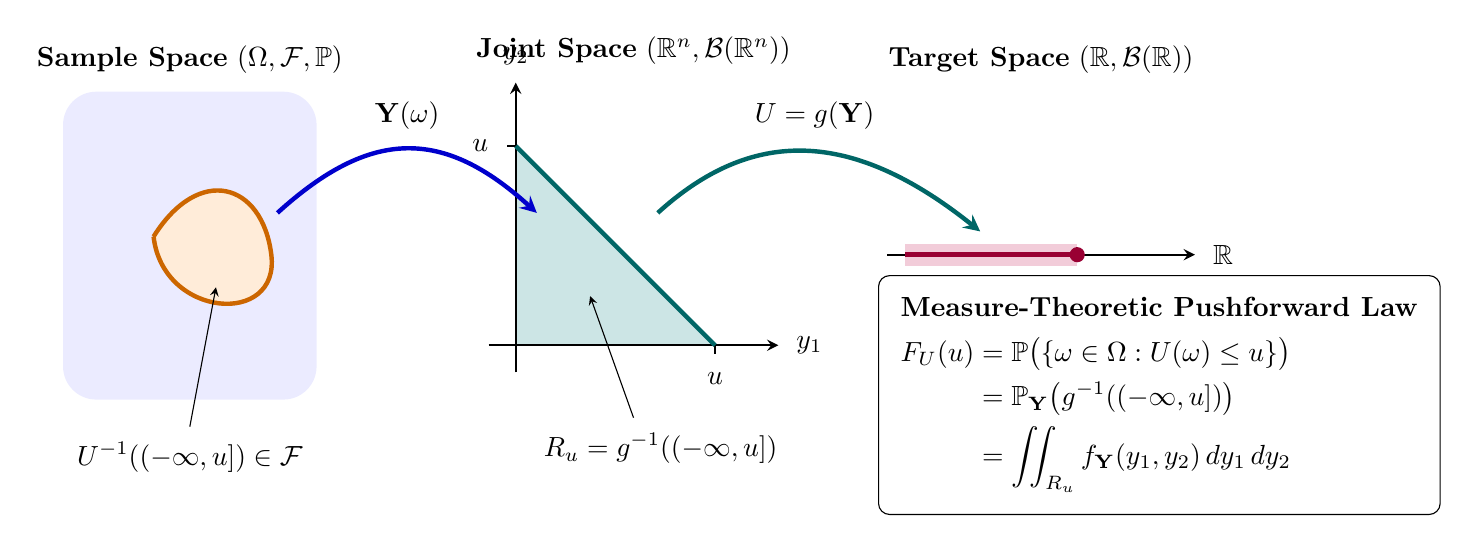
\begin{tikzpicture}[scale=1.15]
    % 1) Backgrounds / Shaded Regions
    \fill[blue!8, rounded corners=12pt] (-4.5, -1.6) rectangle (-1.7, 1.8);
    \fill[orange!15] (-3.5, 0.2) .. controls (-3.0, 1.0) and (-2.3, 0.8) .. (-2.2, 0.0) .. controls (-2.1, -0.8) and (-3.4, -0.7) .. (-3.5, 0.2);
    
    % Shaded Simplex in R^2
    \fill[teal!20] (0.5, -1.0) -- (2.7, -1.0) -- (0.5, 1.2) -- cycle;

    % Shaded Interval on R
    \fill[purple!20] (4.8, -0.12) rectangle (6.7, 0.12);

    % 2) Grid Lines and Coordinate Axes
    \draw[thick, ->, >=stealth, black] (0.2, -1.0) -- (3.4, -1.0);
    \draw[thick, ->, >=stealth, black] (0.5, -1.3) -- (0.5, 1.9);
    \draw[thick, ->, >=stealth, black] (4.6, 0.0) -- (8.0, 0.0);

    % Tick marks (Decoupled Node Buffers)
    \draw[thick, black] (2.7, -1.0) -- (2.7, -1.1) node[below=3pt, text=black] {$u$};
    \draw[thick, black] (0.5, 1.2) -- (0.4, 1.2) node[left=3pt, text=black] {$u$};
    \draw[thick, black] (6.7, 0.08) -- (6.7, -0.08) node[below=4pt, text=black] {$u$};

    % 3) Primary Plots and Mapping Curves
    \draw[ultra thick, orange!80!black] (-3.5, 0.2) .. controls (-3.0, 1.0) and (-2.3, 0.8) .. (-2.2, 0.0) .. controls (-2.1, -0.8) and (-3.4, -0.7) .. (-3.5, 0.2);
    \draw[ultra thick, teal!80!black] (0.5, 1.2) -- (2.7, -1.0);
    \draw[ultra thick, purple!80!black] (4.8, 0.0) -- (6.7, 0.0);
    \filldraw[purple!80!black] (6.7, 0.0) circle (2.2pt);

    % Mapping Arrows between Spaces
    \draw[ultra thick, ->, >=stealth, blue!80!black, shorten >=3pt, shorten <=3pt] (-2.2, 0.4) .. controls (-1.1, 1.4) and (-0.3, 1.4) .. (0.8, 0.4);
    \draw[ultra thick, ->, >=stealth, teal!80!black, shorten >=3pt, shorten <=3pt] (2.0, 0.4) .. controls (3.1, 1.4) and (4.2, 1.4) .. (5.7, 0.2);

    % Off-Axis Callout Arrows
    \draw[->, >=stealth, shorten >=2pt, black] (1.8, -1.8) -- (1.3, -0.4);
    \draw[->, >=stealth, shorten >=2pt, black] (-3.1, -1.9) -- (-2.8, -0.3);

    % 4) Node Labels and Text
    \node[above=3pt, text=black] at (-3.1, 1.8) {\textbf{Sample Space} $(\Omega, \F, \Prob)$};
    \node[above=3pt, text=black] at (1.8, 1.9) {\textbf{Joint Space} $(\R^n, \mathcal{B}(\R^n))$};
    \node[above=3pt, text=black] at (6.3, 1.8) {\textbf{Target Space} $(\R, \mathcal{B}(\R))$};

    \node[right=3pt, text=black] at (3.4, -1.0) {$y_1$};
    \node[above=3pt, text=black] at (0.5, 1.9) {$y_2$};
    \node[right=3pt, text=black] at (8.0, 0.0) {$\R$};

    \node[above=4pt, text=black] at (-0.7, 1.15) {$\displaystyle \mathbf{Y}(\omega)$};
    \node[above=4pt, text=black] at (3.8, 1.15) {$\displaystyle U = g(\mathbf{Y})$};

    % Off-axis callout text nodes
    \node[below=2pt, text=black] at (-3.1, -1.9) {$\displaystyle U^{-1}((-\infty, u]) \in \F$};
    \node[below=2pt, text=black] at (2.1, -1.8) {$\displaystyle R_u = g^{-1}((-\infty, u])$};

    % Single-Node Multiline Legend (Anchor Pivot Strategy)
    \node[draw=black, fill=white, rounded corners=4pt, align=left, inner sep=8pt, anchor=west, text=black] at (4.5, -1.55) {
        \textbf{Measure-Theoretic Pushforward Law}\\[4pt]
        $\displaystyle F_U(u) = \Prob\big(\{\omega \in \Omega : U(\omega) \le u\}\big)$\\[3pt]
        $\displaystyle \phantom{F_U(u)} = \Prob_{\mathbf{Y}}\big(g^{-1}((-\infty, u])\big)$\\[3pt]
        $\displaystyle \phantom{F_U(u)} = \iint_{R_u} f_{\mathbf{Y}}(y_1, y_2)\,dy_1\,dy_2$
    };
\end{tikzpicture}
\end{center}
\begin{center}
\small \textbf{Figure 1:} Visual representation of the composite measurable mapping $U = g \circ \mathbf{Y}: \Omega \to \R^n \to \R$ and the pre-image integration region $R_u = g^{-1}((-\infty, u])$.
\end{center}

\vspace{0.8em}

\begin{center}
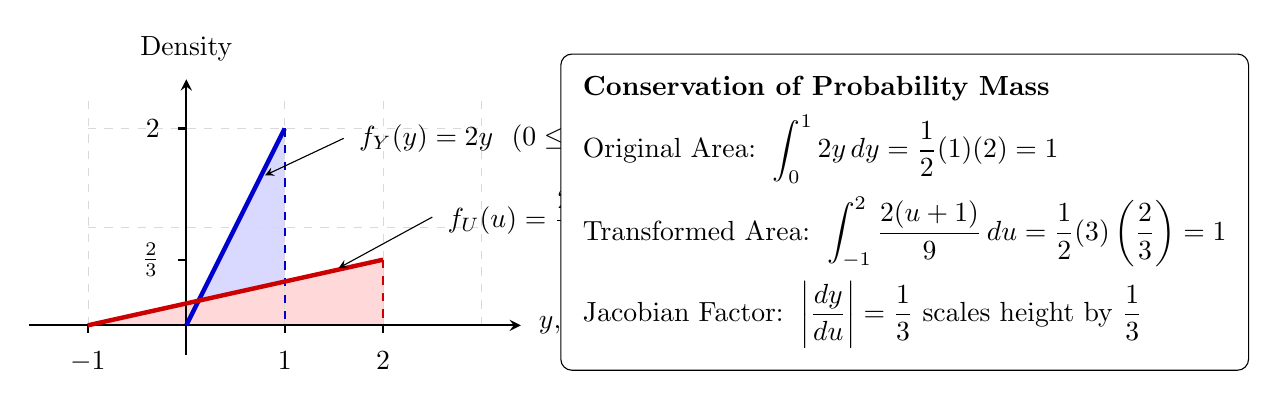
\begin{tikzpicture}[scale=1.25]
    % 1) Backgrounds / Shaded Area under PDFs
    \fill[blue!15] (0.0, 0.0) -- (1.0, 2.0) -- (1.0, 0.0) -- cycle;
    \fill[red!15] (-1.0, 0.0) -- (2.0, 0.667) -- (2.0, 0.0) -- cycle;

    % 2) Grid Lines and Axes
    \draw[help lines, gray!30, dashed] (-1.0, 0.0) grid (3.0, 2.3);
    \draw[thick, ->, >=stealth, black] (-1.6, 0.0) -- (3.4, 0.0);
    \draw[thick, ->, >=stealth, black] (0.0, -0.3) -- (0.0, 2.5);

    % Microscopic Tick Marks (Decoupled Node Buffers)
    \draw[thick, black] (-1.0, 0.0) -- (-1.0, -0.08) node[below=3pt, text=black] {$-1$};
    \draw[thick, black] (1.0, 0.0) -- (1.0, -0.08) node[below=3pt, text=black] {$1$};
    \draw[thick, black] (2.0, 0.0) -- (2.0, -0.08) node[below=3pt, text=black] {$2$};
    \draw[thick, black] (0.0, 2.0) -- (-0.08, 2.0) node[left=3pt, text=black] {$2$};
    \draw[thick, black] (0.0, 0.667) -- (-0.08, 0.667) node[left=3pt, text=black] {$\frac{2}{3}$};

    % 3) Primary Plots (Ultra Thick High-Contrast Curves)
    \draw[ultra thick, blue!80!black] (0.0, 0.0) -- (1.0, 2.0);
    \draw[thick, dashed, blue!80!black] (1.0, 2.0) -- (1.0, 0.0);

    \draw[ultra thick, red!80!black] (-1.0, 0.0) -- (2.0, 0.667);
    \draw[thick, dashed, red!80!black] (2.0, 0.667) -- (2.0, 0.0);

    % Off-Axis Callout Arrows
    \draw[->, >=stealth, shorten >=2pt, black] (1.6, 1.9) -- (0.75, 1.5);
    \draw[->, >=stealth, shorten >=2pt, black] (2.5, 1.1) -- (1.5, 0.556);

    % 4) Node Labels and Text
    \node[right=3pt, text=black] at (3.4, 0.0) {$y, u$};
    \node[above=3pt, text=black] at (0.0, 2.5) {$\text{Density}$};

    \node[right=2pt, text=black] at (1.6, 1.9) {$\displaystyle f_Y(y) = 2y \ \ (0 \le y \le 1)$};
    \node[right=2pt, text=black] at (2.5, 1.1) {$\displaystyle f_U(u) = \frac{2(u+1)}{9} \ \ (-1 \le u \le 2)$};

    % Single-Node Multiline Annotation Block (Anchor Pivot Strategy)
    \node[draw=black, fill=white, rounded corners=4pt, align=left, inner sep=8pt, anchor=west, text=black] at (3.8, 1.15) {
        \textbf{Conservation of Probability Mass}\\[4pt]
        $\displaystyle \text{Original Area: } \int_0^1 2y\,dy = \frac{1}{2}(1)(2) = 1$\\[4pt]
        $\displaystyle \text{Transformed Area: } \int_{-1}^2 \frac{2(u+1)}{9}\,du = \frac{1}{2}(3)\left(\frac{2}{3}\right) = 1$\\[4pt]
        $\displaystyle \text{Jacobian Factor: } \left|\frac{dy}{du}\right| = \frac{1}{3} \text{ scales height by } \frac{1}{3}$
    };
\end{tikzpicture}
\end{center}
\begin{center}
\small \textbf{Figure 2:} Geometric comparison of $f_Y(y) = 2y$ on $[0, 1]$ and $f_U(u) = \frac{2(u+1)}{9}$ on $[-1, 2]$ from Example 6.1 ($U = 3Y - 1$).
\end{center}

\subsection{Heuristics and ``Cheats'' for Method Selection}

\begin{enumerate}[label=\textbf{Heuristic \arabic*:}]
    \item \textbf{The ``Sum of $n$ Independent RVs'' Trigger $\implies$ Always Use Method 3 (MGFs) First}:
    Whenever you see $U = \sum_{i=1}^n Y_i$ or $\bar{Y} = \frac{1}{n}\sum_{i=1}^n Y_i$ where $n \ge 3$ and $Y_i$ belong to the Normal, Gamma, Exponential, Chi-Square, Binomial, or Poisson families, \textit{never} set up an $n$-dimensional integral. Multiply their MGFs in three lines and invoke Theorem 6.1.
    \item \textbf{The ``Even Power or Absolute Value'' Trigger $\implies$ Always Use Method 1 (CDF Method)}:
    If $U = Y^2$, $U = |Y|$, or $U = (Y - c)^2$ on a domain containing $c$, the function folds the real line. Directly write $\Prob(Y^2 \le u) = \Prob(-\sqrt{u} \le Y \le \sqrt{u}) = F_Y(\sqrt{u}) - F_Y(-\sqrt{u})$ and differentiate via the Chain Rule: $f_U(u) = \frac{1}{2\sqrt{u}}\big[f_Y(\sqrt{u}) + f_Y(-\sqrt{u})\big]$ for $u > 0$.
    \item \textbf{The ``Quick Sanity Check''}:
    After deriving any density $f_U(u)$, immediately test two things: (1) Is $f_U(u) \ge 0$ on your stated support? (If it is negative, you forgot the absolute value around the Jacobian!). (2) Does $\int_{\mathcal{S}_U} f_U(u)\,du = 1$? (If it does not integrate to $1$, your support boundaries or integration limits were not properly transformed!).
\end{enumerate}

\subsection{Common Pitfalls and Logical Fallacies}

\begin{itemize}
    \item \textbf{Pitfall 1: The ``Plug-and-Play'' Density Fallacy (Omitting the Jacobian)}:
    A frequent beginner mistake is assuming that if $U = h(Y)$, then $f_U(u) = f_Y(h^{-1}(u))$. This confuses a \textit{scalar function value} with a \textit{differential 1-form} $f_Y(y)\,dy$. A probability density only has meaning when multiplied by the differential volume element $dy = |h^{-1}{'}(u)|\,du$.
    \item \textbf{Pitfall 2: Applying MGF Factorization to Uncorrelated (but Dependent) Variables}:
    The identity $m_{Y_1 + Y_2}(t) = m_{Y_1}(t) m_{Y_2}(t)$ requires full statistical independence, \textit{not} merely zero covariance ($\operatorname{Cov}(Y_1, Y_2) = 0$).
    \item \textbf{Pitfall 3: Leaving Old Variables in the Final Density}:
    A marginal density $f_U(u)$ is a function of $u$ alone. If $y$ or $y_1$ still appears in your final formula for $f_U(u)$ (including inside the piece-wise support inequalities!), the solution is incomplete.
\end{itemize}

\newpage
% ==============================================================================
% PART 5: CONCEPTUAL SYNTHESIS AND THE "BIG PICTURE"
% ==============================================================================
\section{Conceptual Synthesis and the ``Big Picture''}

\subsection{Thematic Connections: Functoriality of Pushforward Measures}

At the highest level of mathematical abstraction, the entire chapter on ``Finding the Probability Distribution of a Function of Random Variables'' is the study of the \textbf{pushforward functor} in the category $\mathbf{Meas}$ of measurable spaces. Given a chain of measurable mappings:
\[
    (\Omega, \F, \Prob) \xrightarrow{\;\mathbf{Y}\;} \big(\R^n, \mathcal{B}(\R^n), \Prob_{\mathbf{Y}}\big) \xrightarrow{\;g\;} \big(\R^m, \mathcal{B}(\R^m), \Prob_{\mathbf{U}}\big),
\]
the pushforward operation satisfies the covariant functorial identity $(g \circ \mathbf{Y})_\# \Prob = g_\# (\mathbf{Y}_\# \Prob)$. Every method in Section 6.2 is simply a different representation of this single measure-theoretic invariant:
\begin{enumerate}[label=(\roman*)]
    \item \textbf{Method 1 (CDF Method)} evaluates the pushforward measure $\Prob_{\mathbf{U}}((-\infty, u]) = \Prob_{\mathbf{Y}}(g^{-1}((-\infty, u]))$ directly on the generating $\pi$-system of half-infinite intervals.
    \item \textbf{Method 2 (Transformation Method)} computes the Radon-Nikodym derivative $\frac{d(g_\# \Prob_{\mathbf{Y}})}{d\lambda}$ directly via the Chain Rule for Radon-Nikodym derivatives: $\frac{d\Prob_U}{d\lambda}(u) = \frac{d\Prob_Y}{d\lambda}(h^{-1}(u)) \cdot \frac{d(h_\# \lambda)}{d\lambda}(u)$.
    \item \textbf{Method 3 (MGF Method)} utilizes the dual Banach space of bounded continuous exponential test functions $e^{tu}$, exploiting the Riesz Representation and Laplace-Fourier isomorphism between measures and their integral transforms.
\end{enumerate}

\subsection{Forward and Backward Links Across Mathematics}

\begin{itemize}
    \item \textbf{Backward Links}:
    \begin{itemize}
        \item \textit{Single and Multivariable Calculus}: The univariate Method of Transformations is precisely the Change of Variables Theorem ($u$-substitution) in reverse, while Method 4 is the $n$-dimensional Jacobian theorem for multiple integrals.
        \item \textit{Foundational Set Theory}: The validity of Method 1 rests entirely on the fact that pre-images preserve all Boolean set operations: $g^{-1}(A^c) = (g^{-1}(A))^c$ and $g^{-1}(\bigcup A_i) = \bigcup g^{-1}(A_i)$.
    \end{itemize}
    \item \textbf{Forward Links}:
    \begin{itemize}
        \item \textit{Mathematical Statistics (Sampling Distributions \& Hypothesis Testing)}: In Chapter 7 of Wackerly et al., these exact three methods are used to prove that for a normal random sample $Y_1, \dots, Y_n \sim \mathcal{N}(\mu, \sigma^2)$, the scaled sample variance $\frac{(n-1)S^2}{\sigma^2} \sim \chi^2_{n-1}$ (via MGFs and Cochran's Theorem), Student's $T = \frac{\sqrt{n}(\bar{Y}-\mu)/ \sigma}{\sqrt{S^2/\sigma^2}} \sim t_{n-1}$ (via Bivariate Transformation), and Snedecor's $F = \frac{S_1^2/\sigma_1^2}{S_2^2/\sigma_2^2} \sim F_{\nu_1, \nu_2}$.
        \item \textit{Asymptotic Theory (Central Limit Theorem)}: Method 3 (MGFs / Characteristic Functions) is the exact tool used to prove that the standardized sample mean $Z_n = \frac{\sqrt{n}(\bar{Y}_n - \mu)}{\sigma} \xrightarrow{d} \mathcal{N}(0, 1)$ by Taylor-expanding $\ln m_{Z_n}(t) = \frac{t^2}{2} + O(n^{-1/2})$.
        \item \textit{Stochastic Calculus (Itô's Lemma)}: When a random variable $Y$ is generalized to a continuous-time stochastic process $X_t$ driven by Brownian motion $W_t$, the classical Method of Transformations generalizes to \textbf{Itô's Formula}, where the non-vanishing quadratic variation $(dW_t)^2 = dt$ adds a second-order curvature drift term $\frac{1}{2}g''(X_t)(dX_t)^2$.
    \end{itemize}

\newpage
% ==============================================================================
% PART 6: ABSTRACT REAL-WORLD MODELING (AI, ML, & QUANT FINANCE)
% ==============================================================================
\section{Abstract Real-World Modeling (AI, ML, and Quantitative Finance)}

\subsection{Concrete Advanced Scenarios}

\subsubsection*{Scenario 1: Generative AI \& Deep Learning -- Normalizing Flows and VAEs}
In modern Deep Generative Modeling, a core objective is to learn a complex, high-dimensional probability density $p_{\mathbf{X}}(\mathbf{x})$ (such as the distribution of high-resolution images or molecular conformations in $\R^d$). **Normalizing Flows** (e.g., RealNVP, Glow, Neural Spline Flows) construct $\mathbf{X}$ as a composite transformation of a simple latent Gaussian vector $\mathbf{Z} \sim \mathcal{N}(\mathbf{0}, I_d)$ through a sequence of $K$ learnable neural diffeomorphisms $\mathbf{X} = \mathbf{h}_K \circ \mathbf{h}_{K-1} \circ \cdots \circ \mathbf{h}_1(\mathbf{Z})$. By **Method 2 / Method 4 (Multivariate Method of Transformations)**, the exact log-likelihood of a data point $\mathbf{x}$ is given by the Change of Variables Theorem:
\[
    \ln p_{\mathbf{X}}(\mathbf{x}; \theta) = \ln p_{\mathbf{Z}}\big(\mathbf{h}_\theta^{-1}(\mathbf{x})\big) + \sum_{k=1}^K \ln \left| \det \frac{\partial \mathbf{h}_{k}^{-1}}{\partial \mathbf{z}_k} \right|.
\]
Similarly, in **Variational Autoencoders (VAEs)**, training via stochastic gradient descent requires differentiating an expectation $\E_{q_\phi(\mathbf{z}|\mathbf{x})}[\mathcal{L}(\mathbf{z})]$ with respect to the distribution parameters $\phi = (\boldsymbol{\mu}, \boldsymbol{\sigma})$. Kingma and Welling's **Reparameterization Trick** expresses $\mathbf{Z} = \boldsymbol{\mu}_\phi(\mathbf{x}) + \boldsymbol{\sigma}_\phi(\mathbf{x}) \odot \boldsymbol{\epsilon}$ where $\boldsymbol{\epsilon} \sim \mathcal{N}(\mathbf{0}, I)$ is a parameter-free base random variable---a direct application of representing a random variable as a deterministic transformation of another random variable!

\subsubsection*{Scenario 2: Quantitative Finance -- Option Pricing and Risk-Neutral Densities}
In quantitative derivatives pricing, the terminal price $S_T$ of an equity or foreign exchange asset at maturity $T$ is modeled as an exponential function of an arithmetic Brownian motion $W_T \sim \mathcal{N}(0, T)$:
\[
    S_T = g(W_T) = S_0 \exp\left(\left(r - \frac{1}{2}\sigma^2\right)T + \sigma W_T\right).
\]
Determining the no-arbitrage price of a European Call Option $C_0 = e^{-rT}\E^{\mathbb{Q}}[\max(S_T - K, 0)]$ requires finding the exact probability density $f_{S_T}(s)$ of the transformed random variable $S_T = g(W_T)$ via the Method of Transformations, and then evaluating the truncated expectation of the piecewise non-monotonic payoff function $U = \max(S_T - K, 0)$ via the Method of Distribution Functions.

\subsubsection*{Scenario 3: Statistical Learning Theory -- Chernoff Concentration Bounds for Empirical Risk}
In Machine Learning theory, given $n$ i.i.d.\ training examples $Z_1, \dots, Z_n$, the empirical risk of a hypothesis $h$ is the sample mean $\hat{R}_n(h) = \frac{1}{n}\sum_{i=1}^n \ell(h, Z_i)$ of the bounded loss variables $Y_i = \ell(h, Z_i)$ with true population risk $\mu = R(h)$. Directly echoing Page 297 of our text ("determine the probability that the error of estimation $|\bar{Y} - \mu|$ is less than or equal to $B$"), **Method 3 (The Method of Moment-Generating Functions)** combined with Markov's inequality yields the celebrated **Chernoff-Hoeffding Bound**:
\[
    \Prob(\bar{Y} - \mu \ge B) = \Prob\big(e^{t(\bar{Y} - \mu)} \ge e^{tB}\big) \le e^{-t(\mu + B)} m_{\bar{Y}}(t) = e^{-t(\mu + B)} \prod_{i=1}^n m_{Y_i}\left(\frac{t}{n}\right) \le \exp\left(-\frac{2nB^2}{(b-a)^2}\right).
\]

\subsection{Rigorous Quantitative Research Model: Stochastic Calculus Meets Normalizing Flows}

We now formulate a complete, research-grade mathematical model uniting Stochastic Differential Equations (SDEs), the Method of Transformations, and Deep Normalizing Flows for pricing exotic options.

\subsubsection*{1. State Space and Filtered Probability Space}
Let $(\Omega, \F, (\F_t)_{t \in [0, T]}, \mathbb{Q})$ be a complete filtered probability space satisfying the usual conditions, where $\mathbb{Q}$ is the unique equivalent martingale (risk-neutral) measure, and $(W_t)_{t \in [0, T]}$ is a standard 1-dimensional $\F_t$-Brownian motion such that $W_T \sim \mathcal{N}(0, T)$ has density:
\[
    f_{W_T}(w) = \frac{1}{\sqrt{2\pi T}} \exp\left(-\frac{w^2}{2T}\right), \quad w \in \R.
\]

\subsubsection*{2. Stochastic Differential Equation and Itô's Transformation}
Suppose the underlying asset price process $(S_t)_{t \in [0, T]}$ evolves according to Geometric Brownian Motion:
\[
    dS_t = r S_t \, dt + \sigma S_t \, dW_t, \qquad S_0 > 0,
\]
where $r \in \R$ is the constant risk-free interest rate and $\sigma > 0$ is the volatility. Define the logarithmic transformation $Y_t = h(S_t) = \ln S_t$. Since $h'(s) = \frac{1}{s}$ and $h''(s) = -\frac{1}{s^2}$, **Itô's Lemma** (the stochastic differential extension of the Method of Transformations) yields:
\[
    d(\ln S_t) = \frac{1}{S_t} dS_t + \frac{1}{2}\left(-\frac{1}{S_t^2}\right) (dS_t)^2 = \frac{1}{S_t}(r S_t \, dt + \sigma S_t \, dW_t) - \frac{1}{2 S_t^2}(\sigma^2 S_t^2 \, dt) = \left(r - \frac{1}{2}\sigma^2\right) dt + \sigma \, dW_t.
\]
Integrating from $t = 0$ to $t = T$ and exponentiating expresses $S_T$ as an explicit strictly increasing transformation of $W_T$:
\[
    S_T = H(W_T) \coloneqq S_0 \exp\left(\left(r - \frac{1}{2}\sigma^2\right)T + \sigma W_T\right).
\]

\subsubsection*{3. Exact Derivation of the Risk-Neutral Density via Method 2}
Since $H: \R \to (0, \infty)$ is strictly increasing ($\frac{dH}{dw} = \sigma H(w) > 0$), we invert $s = H(w)$ for $s > 0$:
\[
    w = H^{-1}(s) = \frac{\ln(s / S_0) - \left(r - \frac{1}{2}\sigma^2\right)T}{\sigma}, \qquad \left|\frac{d}{ds} H^{-1}(s)\right| = \frac{1}{\sigma s}.
\]
Applying **Theorem \ref{thm:transformation_method} (Method of Transformations)**, the exact risk-neutral PDF of $S_T$ is the Log-Normal density:
\[
    f_{S_T}(s) = f_{W_T}\big(H^{-1}(s)\big) \left|\frac{d}{ds} H^{-1}(s)\right| = \frac{1}{s \sigma \sqrt{2\pi T}} \exp\left( -\frac{\left[\ln(s / S_0) - \left(r - \frac{1}{2}\sigma^2\right)T\right]^2}{2\sigma^2 T} \right) \mathbf{1}_{(0, \infty)}(s).
\]

\subsubsection*{4. Neural Normalizing Flow Optimization for Implied Volatility Smile}
In real financial markets, the true terminal return $X_T = \ln(S_T / S_0)$ exhibits heavy tails and skewness not captured by a simple Gaussian. We model $X_T = \Phi_\theta(Z)$ where $Z \sim \mathcal{N}(0, 1)$ and $\Phi_\theta: \R \to \R$ is a strictly monotonic neural network parameterized by weights $\theta$ (with $\frac{\partial \Phi_\theta}{\partial z} > 0$). By the Method of Transformations, the model-implied terminal asset density is:
\[
    q_\theta(s) = \frac{1}{s} \varphi\big(\Phi_\theta^{-1}(\ln(s / S_0))\big) \left( \frac{\partial \Phi_\theta}{\partial z}\Big|_{z = \Phi_\theta^{-1}(\ln(s/S_0))} \right)^{-1},
\]
where $\varphi(z) = \frac{1}{\sqrt{2\pi}}e^{-z^2/2}$. Given observed market prices $\{\hat{C}_j\}_{j=1}^M$ of European call options at strikes $\{K_j\}_{j=1}^M$, the calibration problem is formulated as the constrained variational optimization problem:
\[
    \min_{\theta} \; \mathcal{L}(\theta) = \sum_{j=1}^M \left( e^{-rT} \int_{-\infty}^{\infty} \max\big(S_0 e^{\Phi_\theta(z)} - K_j, 0\big) \varphi(z) \, dz - \hat{C}_j \right)^2 + \lambda_{\text{mart}} \left( \int_{-\infty}^{\infty} e^{\Phi_\theta(z)} \varphi(z) \, dz - e^{rT} \right)^2,
\]
where the second term enforces the martingale no-arbitrage constraint $\E^{\mathbb{Q}}[S_T] = S_0 e^{rT}$ via LOTUS.

\newpage
% ==============================================================================
% PART 7: COMMON VARIATIONS AND UNTESTED CONCEPTS
% ==============================================================================
\section{Common Variations and Untested Concepts}

While the provided textbook excerpt introduces the overview of the three primary methods and a linear univariate example, standard university examinations on Chapter 6 heavily test three advanced variations that are omitted from the introductory excerpt: (1) **Order Statistics** ($Y_{(1)}, \dots, Y_{(n)}$), (2) **The Multivariate Jacobian Method (Section 6.6)**, and (3) **Mixed Discrete-Continuous Transformations (Rectified / Censored Random Variables)**. We provide rigorous derivations of each below.

\subsection{Untested Concept 1: Probability Distributions of Order Statistics}

\begin{theorem}[Minimum, Maximum, and $k$-th Order Statistic of a Random Sample]
Let $Y_1, Y_2, \dots, Y_n$ be a continuous random sample of size $n$ with common CDF $F(y)$ and common PDF $f(y)$. Let $Y_{(1)} \le Y_{(2)} \le \cdots \le Y_{(n)}$ denote the sorted random variables (\textbf{order statistics}), where $Y_{(1)} = \min(Y_1, \dots, Y_n)$ and $Y_{(n)} = \max(Y_1, \dots, Y_n)$. Then:
\[
    f_{Y_{(n)}}(y) = n \big[F(y)\big]^{n-1} f(y), \qquad f_{Y_{(1)}}(y) = n \big[1 - F(y)\big]^{n-1} f(y),
\]
and in general, for the $k$-th order statistic $Y_{(k)}$ ($1 \le k \le n$):
\[
    f_{Y_{(k)}}(y) = \frac{n!}{(k-1)!(n-k)!} \big[F(y)\big]^{k-1} \big[1 - F(y)\big]^{n-k} f(y).
\]
\end{theorem}

\begin{proof}
We use **Method 1 (The Method of Distribution Functions)**:
\begin{enumerate}[label=\textbf{Step \arabic*:}]
    \item \textit{Maximum $Y_{(n)}$}: The event $\{\max(Y_1, \dots, Y_n) \le y\}$ occurs if and only if \textit{every} $Y_i \le y$:
    \[
        F_{Y_{(n)}}(y) = \Prob(Y_{(n)} \le y) = \Prob(Y_1 \le y, Y_2 \le y, \dots, Y_n \le y) = \prod_{i=1}^n \Prob(Y_i \le y) = \big[F(y)\big]^n.
    \]
    Differentiating with respect to $y$ via the Chain Rule gives $f_{Y_{(n)}}(y) = \frac{d}{dy}\big[F(y)\big]^n = n\big[F(y)\big]^{n-1} f(y)$.
    \item \textit{Minimum $Y_{(1)}$}: The complementary event $\{\min(Y_1, \dots, Y_n) > y\}$ occurs if and only if \textit{every} $Y_i > y$:
    \[
        F_{Y_{(1)}}(y) = 1 - \Prob(Y_{(1)} > y) = 1 - \Prob(Y_1 > y, \dots, Y_n > y) = 1 - \prod_{i=1}^n \big[1 - F(y)\big] = 1 - \big[1 - F(y)\big]^n.
    \]
    Differentiating with respect to $y$ gives $f_{Y_{(1)}}(y) = -n\big[1 - F(y)\big]^{n-1}(-f(y)) = n\big[1 - F(y)\big]^{n-1} f(y)$.
    \item \textit{General $Y_{(k)}$}: Note that $\{Y_{(k)} \le y\}$ occurs if and only if \textit{at least $k$} of the $n$ independent random variables $Y_1, \dots, Y_n$ are less than or equal to $y$. Since each trial $\mathbf{1}_{\{Y_i \le y\}}$ is an independent Bernoulli trial with success probability $p = F(y)$, the number of variables $\le y$ follows a $\operatorname{Binomial}(n, F(y))$ distribution:
    \[
        F_{Y_{(k)}}(y) = \sum_{j=k}^n \binom{n}{j} \big[F(y)\big]^j \big[1 - F(y)\big]^{n-j}.
    \]
    Differentiating term-by-term with respect to $y$ produces a telescoping sum where all terms cancel except the boundary term $j = k$, yielding $f_{Y_{(k)}}(y) = \frac{n!}{(k-1)!(n-k)!}[F(y)]^{k-1}[1-F(y)]^{n-k}f(y)$.
\end{enumerate}
\end{proof}

\subsection{Untested Concept 2: The Multivariate Jacobian Method (Gamma-Beta Decoupling)}

\begin{example}[Joint Transformation of Independent Exponential Variables]
Let $Y_1, Y_2 \stackrel{\text{i.i.d.}}{\sim} \operatorname{Exp}(1)$ with joint density $f_{Y_1, Y_2}(y_1, y_2) = e^{-(y_1 + y_2)}$ for $y_1 > 0, y_2 > 0$. Define the bivariate transformation:
\[
    U_1 = Y_1 + Y_2, \qquad U_2 = \frac{Y_1}{Y_1 + Y_2}.
\]
Find the joint PDF $f_{U_1, U_2}(u_1, u_2)$ and prove that $U_1$ and $U_2$ are statistically independent.
\end{example}

\begin{proof}[Solution via Method 4 (Multivariate Jacobians)]
\begin{enumerate}[label=\textbf{Step \arabic*:}]
    \item \textit{Invert the Transformation and Map the Support}: From $u_1 = y_1 + y_2$ and $u_2 = \frac{y_1}{u_1}$, we solve uniquely for $(y_1, y_2)$:
    \[
        y_1 = w_1(u_1, u_2) = u_1 u_2, \qquad y_2 = w_2(u_1, u_2) = u_1(1 - u_2).
    \]
    The original support $y_1 > 0, y_2 > 0$ maps to $u_1 u_2 > 0$ and $u_1(1 - u_2) > 0$, which is equivalent to the rectangular product support:
    \[
        \mathcal{S}_{\mathbf{U}} = \{(u_1, u_2) \in \R^2 : u_1 > 0, \ 0 < u_2 < 1\} = (0, \infty) \times (0, 1).
    \]
    \item \textit{Compute the Jacobian Determinant}:
    \[
        \det J(u_1, u_2) = \det \begin{pmatrix} \dfrac{\partial y_1}{\partial u_1} & \dfrac{\partial y_1}{\partial u_2} \\[10pt] \dfrac{\partial y_2}{\partial u_1} & \dfrac{\partial y_2}{\partial u_2} \end{pmatrix} = \det \begin{pmatrix} u_2 & u_1 \\ 1 - u_2 & -u_1 \end{pmatrix} = -u_1 u_2 - u_1(1 - u_2) = -u_1.
    \]
    Taking the absolute value gives $|\det J(u_1, u_2)| = |-u_1| = u_1$ (since $u_1 > 0$).
    \item \textit{Substitute into Theorem \ref{thm:jacobian}}:
    \[
        f_{U_1, U_2}(u_1, u_2) = f_{Y_1, Y_2}\big(u_1 u_2, u_1(1 - u_2)\big) \cdot |\det J| = e^{-(u_1 u_2 + u_1(1 - u_2))} \cdot u_1 = u_1 e^{-u_1} \cdot 1,
    \]
    for $u_1 > 0$ and $0 < u_2 < 1$. Because the support $(0, \infty) \times (0, 1)$ is a Cartesian product and the joint density factors into $f_{U_1}(u_1) = u_1 e^{-u_1} \mathbf{1}_{(0,\infty)}(u_1)$ ($\operatorname{Gamma}(2,1)$) and $f_{U_2}(u_2) = 1 \cdot \mathbf{1}_{(0,1)}(u_2)$ ($\operatorname{Uniform}(0,1) = \operatorname{Beta}(1,1)$), $U_1$ and $U_2$ are mutually independent!
\end{enumerate}
\end{proof}

\subsection{Untested Concept 3: Mixed Discrete-Continuous Transformations (ReLU / Censoring)}

\begin{example}[Distribution of a Rectified Linear Unit $U = \max(0, Y)$]
Let $Y \sim \mathcal{N}(0, 1)$ be a standard normal random variable, and let $U = \max(0, Y)$ (the Rectified Linear Unit activation function in Deep Neural Networks, or a censored payoff). Find the exact CDF $F_U(u)$ and show that $U$ is neither purely discrete nor purely continuous.
\end{example}

\begin{proof}[Solution via Method 1 (Method of Distribution Functions)]
We evaluate $F_U(u) = \Prob(\max(0, Y) \le u)$ across three regimes:
\begin{itemize}
    \item \textbf{Case 1 ($u < 0$)}: Since $\max(0, Y) \ge 0$ for all $\omega \in \Omega$, the event $\{\max(0, Y) \le u\}$ is the empty set $\emptyset$ when $u < 0$. Thus $F_U(u) = \Prob(\emptyset) = 0$.
    \item \textbf{Case 2 ($u = 0$)}: $\max(0, Y) \le 0 \iff Y \le 0$. Thus:
    \[
        F_U(0) = \Prob(Y \le 0) = \Phi(0) = \frac{1}{2}.
    \]
    Notice that $\lim_{u \to 0^-} F_U(u) = 0 \neq \frac{1}{2} = F_U(0)$. Thus $F_U(u)$ has a jump discontinuity of size $\frac{1}{2}$ at $u = 0$, corresponding to a discrete point mass $\Prob(U = 0) = \frac{1}{2}$!
    \item \textbf{Case 3 ($u > 0$)}: For $u > 0$, $\max(0, Y) \le u \iff (0 \le u \text{ and } Y \le u) \iff Y \le u$. Thus:
    \[
        F_U(u) = \Prob(Y \le u) = \Phi(u) = \int_{-\infty}^u \frac{1}{\sqrt{2\pi}} e^{-y^2/2} \, dy, \quad u > 0.
    \]
\end{itemize}
By the Lebesgue Decomposition Theorem, the pushforward measure $\Prob_U$ decomposes into a discrete Dirac measure and an absolutely continuous measure: $d\Prob_U(u) = \frac{1}{2}\delta_0(du) + \frac{1}{\sqrt{2\pi}}e^{-u^2/2}\mathbf{1}_{(0, \infty)}(u)\,du$.
\end{proof}

\newpage
% ==============================================================================
% PART 8: ADVANCED DIAGNOSTIC TESTING: "FIND THE FLAW"
% ==============================================================================
\section{Advanced Diagnostic Testing: ``Find the Flaw''}

Below are five advanced problems accompanied by seemingly rigorous step-by-step solutions. However, \textbf{each proof contains a single, subtle, yet fatal mathematical flaw}. Act as the grader: identify the exact line where the error occurs, explain what theorem or measure-theoretic condition was violated, and write out the corrected derivation. The true resolutions are provided in Section 8.2.

\subsection{The Five Flawed Proofs}

\subsubsection*{Diagnostic Problem 1: The Asymmetric Quadratic Transformation}
\textbf{Problem:} Let $Y$ have a Uniform distribution on $[-1, 2]$, so $f_Y(y) = \frac{1}{3}$ for $-1 \le y \le 2$ and $0$ elsewhere. Find the probability density function $f_U(u)$ of $U = Y^2$.

\textbf{Proposed ``Proof'':}
\begin{enumerate}[label=\textbf{Line \arabic*:}]
    \item Since $y \in [-1, 2]$, the minimum of $u = y^2$ is $0^2 = 0$ and the maximum is $2^2 = 4$, so $u \in [0, 4]$.
    \item For any $u \in (0, 4]$, the equation $u = y^2$ has two inverse branches: $y_1 = -\sqrt{u}$ and $y_2 = +\sqrt{u}$, with derivatives $\left|\frac{dy_1}{du}\right| = \left|\frac{dy_2}{du}\right| = \frac{1}{2\sqrt{u}}$.
    \item By the piecewise monotone Method of Transformations, we sum over both branches for all $u \in (0, 4]$:
    \[
        f_U(u) = f_Y(\sqrt{u})\frac{1}{2\sqrt{u}} + f_Y(-\sqrt{u})\frac{1}{2\sqrt{u}} = \frac{1}{3}\cdot\frac{1}{2\sqrt{u}} + \frac{1}{3}\cdot\frac{1}{2\sqrt{u}} = \frac{1}{3\sqrt{u}}, \quad 0 < u \le 4. \quad \blacksquare
    \]
\end{enumerate}

\subsubsection*{Diagnostic Problem 2: MGF of the Sum of Uncorrelated Normal Variables}
\textbf{Problem:} Let $Y_1 \sim \mathcal{N}(0, 1)$, and let $S$ be an independent Rademacher random variable with $\Prob(S = 1) = \Prob(S = -1) = \frac{1}{2}$. Define $Y_2 = S Y_1$. Find the distribution of $U = Y_1 + Y_2$.

\textbf{Proposed ``Proof'':}
\begin{enumerate}[label=\textbf{Line \arabic*:}]
    \item By symmetry of the standard normal distribution, for any $y \in \R$, $\Prob(Y_2 \le y) = \frac{1}{2}\Prob(Y_1 \le y) + \frac{1}{2}\Prob(-Y_1 \le y) = \Phi(y)$, so $Y_2 \sim \mathcal{N}(0, 1)$ with MGF $m_{Y_2}(t) = e^{t^2/2}$.
    \item Furthermore, $\operatorname{Cov}(Y_1, Y_2) = \E[S Y_1^2] - \E[Y_1]\E[Y_2] = \E[S]\E[Y_1^2] - 0 = 0 \cdot 1 = 0$, so $Y_1$ and $Y_2$ are uncorrelated normal random variables.
    \item Applying Method 3 (the MGF Method) to $U = Y_1 + Y_2$:
    \[
        m_U(t) = m_{Y_1}(t) \cdot m_{Y_2}(t) = e^{t^2/2} \cdot e^{t^2/2} = e^{t^2} = \exp\left(0\cdot t + \frac{1}{2}(2)t^2\right).
    \]
    \item By Theorem 6.1 (Uniqueness of MGFs), $U = Y_1 + Y_2 \sim \mathcal{N}(0, 2)$. $\blacksquare$
\end{enumerate}

\subsubsection*{Diagnostic Problem 3: Bivariate Transformation of a Difference}
\textbf{Problem:} Let $Y_1, Y_2$ be a random sample of size $2$ from $f(y) = e^{-y}$ for $y \ge 0$. Find the PDF of $U = Y_1 - Y_2$.

\textbf{Proposed ``Proof'':}
\begin{enumerate}[label=\textbf{Line \arabic*:}]
    \item By independence, the joint density of $(Y_1, Y_2)$ is $f(y_1, y_2) = e^{-(y_1 + y_2)}$ for $y_1 \ge 0, y_2 \ge 0$.
    \item Using Method 2 (Bivariate Transformations), fix $y_2 \ge 0$ and let $u = y_1 - y_2$, so $y_1 = u + y_2$ and $\left|\frac{\partial y_1}{\partial u}\right| = 1$. Since $Y_1 \ge 0$ and $Y_2 \ge 0$, the difference $U = Y_1 - Y_2$ can take any real value $u \in (-\infty, \infty)$.
    \item Substituting $y_1 = u + y_2$ into the joint density and integrating over $y_2 \in [0, \infty)$ gives:
    \[
        f_U(u) = \int_0^{\infty} f_{Y_1, Y_2}(u + y_2, y_2) \cdot 1 \, dy_2 = \int_0^{\infty} e^{-(u + 2y_2)} \, dy_2 = e^{-u} \int_0^{\infty} e^{-2y_2} \, dy_2 = \frac{1}{2} e^{-u}, \quad u \in \R. \quad \blacksquare
    \]
\end{enumerate}

\subsubsection*{Diagnostic Problem 4: Uniqueness Theorem Applied to Log-Normal Moments}
\textbf{Problem:} Let $Y \sim \mathcal{N}(0, 1)$ and let $U = e^Y$ (the Log-Normal distribution) with density $f_U(u) = \frac{1}{u\sqrt{2\pi}} e^{-(\ln u)^2 / 2}$ for $u > 0$. Consider a second continuous random variable $V$ with density $f_V(u) = f_U(u)\big[1 + \sin(2\pi \ln u)\big]$ for $u > 0$. Prove that $U$ and $V$ have identical moments of all orders ($\E[U^k] = \E[V^k]$ for all $k \in \N$) and deduce by Theorem 6.1 that $f_U = f_V$.

\textbf{Proposed ``Proof'':}
\begin{enumerate}[label=\textbf{Line \arabic*:}]
    \item For any integer $k \ge 1$, substituting $y = \ln u$ ($du = e^y dy$) into the integral for $\E[V^k] - \E[U^k]$ gives:
    \[
        \int_0^{\infty} u^k f_U(u) \sin(2\pi \ln u) \, du = \frac{1}{\sqrt{2\pi}} \int_{-\infty}^{\infty} e^{ky} e^{-y^2/2} \sin(2\pi y) \, dy = \frac{e^{k^2/2}}{\sqrt{2\pi}} \int_{-\infty}^{\infty} e^{-(y-k)^2/2} \sin(2\pi(y - k)) \, dy = 0,
    \]
    because the integrand $w \mapsto e^{-w^2/2}\sin(2\pi w)$ is an odd function integrated over $(-\infty, \infty)$. Thus $\E[U^k] = \E[V^k] = e^{k^2/2}$ for all $k = 0, 1, 2, \dots$.
    \item Expanding the Moment-Generating Functions of $U$ and $V$ in Maclaurin series gives:
    \[
        m_U(t) = \sum_{k=0}^{\infty} \frac{\E[U^k]}{k!} t^k = \sum_{k=0}^{\infty} \frac{\E[V^k]}{k!} t^k = m_V(t).
    \]
    \item By Theorem 6.1 (Uniqueness of MGFs), $U$ and $V$ must have the exact same probability distribution! $\blacksquare$
\end{enumerate}

\subsubsection*{Diagnostic Problem 5: Differentiating an Iterated CDF Integral via Leibniz's Rule}
\textbf{Problem:} Let $(Y_1, Y_2)$ have continuous joint PDF $f(y_1, y_2)$ supported on $y_1 \ge 0, y_2 \ge 0$. Find an integral expression for the PDF $f_U(u)$ of $U = Y_1 + Y_2$ for $u > 0$ using Method 1.

\textbf{Proposed ``Proof'':}
\begin{enumerate}[label=\textbf{Line \arabic*:}]
    \item By Method 1, the CDF of $U$ for $u > 0$ is given by the iterated integral:
    \[
        F_U(u) = \Prob(Y_1 + Y_2 \le u) = \int_0^u \left( \int_0^{u - y_1} f(y_1, y_2) \, dy_2 \right) dy_1.
    \]
    \item Define the inner integral as $G(y_1) = \int_0^{u - y_1} f(y_1, y_2) \, dy_2$, so that $F_U(u) = \int_0^u G(y_1) \, dy_1$.
    \item By the Fundamental Theorem of Calculus, differentiating $F_U(u) = \int_0^u G(y_1) \, dy_1$ with respect to the upper limit $u$ yields $f_U(u) = G(u) = \int_0^{u - u} f(u, y_2) \, dy_2 = 0$. $\blacksquare$
\end{enumerate}

\subsection{Solution Key: Explanations and Corrected Proofs}

\begin{enumerate}[label=\textbf{Resolution \arabic*:}]
    \item \textbf{Flaw in Diagnostic Problem 1 (Line 3 -- Asymmetric Support Violation)}:
    \begin{itemize}
        \item \textit{Why it is an error}: While $y_1 = -\sqrt{u}$ and $y_2 = +\sqrt{u}$ are both valid algebraic solutions to $u = y^2$, the original density $f_Y(y) = \frac{1}{3}$ is only non-zero for $y \in [-1, 2]$. For $u \in (1, 4]$, the negative branch $y_1 = -\sqrt{u}$ falls in $[-2, -1)$, which is \textbf{outside} the support of $Y$, so $f_Y(-\sqrt{u}) = 0$ for $1 < u \le 4$! Notice that integrating the flawed density gives $\int_0^4 \frac{1}{3\sqrt{u}}\,du = \frac{4}{3} \neq 1$.
        \item \textit{Corrected Step}: Split the support of $U$ into $(0, 1]$ (where both branches are active) and $(1, 4]$ (where only the positive branch $y_2 = \sqrt{u} \in (1, 2]$ is active):
        \[
            f_U(u) = \begin{cases}
                \displaystyle \frac{1}{3}\cdot\frac{1}{2\sqrt{u}} + \frac{1}{3}\cdot\frac{1}{2\sqrt{u}} = \frac{1}{3\sqrt{u}}, & 0 < u \le 1, \\[8pt]
                \displaystyle \frac{1}{3}\cdot\frac{1}{2\sqrt{u}} + 0 = \frac{1}{6\sqrt{u}}, & 1 < u \le 4, \\[6pt]
                0, & \text{elsewhere.}
            \end{cases}
        \]
        Now $\int_0^1 \frac{1}{3\sqrt{u}}\,du + \int_1^4 \frac{1}{6\sqrt{u}}\,du = \frac{2}{3}(1) + \frac{1}{3}(2 - 1) = 1$.
    \end{itemize}

    \item \textbf{Flaw in Diagnostic Problem 2 (Line 3 -- False Independence Assumption)}:
    \begin{itemize}
        \item \textit{Why it is an error}: Line 3 writes $m_{Y_1 + Y_2}(t) = m_{Y_1}(t) m_{Y_2}(t)$. However, the expectation of a product equals the product of expectations ($\E[e^{tY_1} e^{tY_2}] = \E[e^{tY_1}]\E[e^{tY_2}]$) \textbf{only when $Y_1$ and $Y_2$ are independent}. Even though $Y_1 \sim \mathcal{N}(0, 1)$, $Y_2 \sim \mathcal{N}(0, 1)$, and $\operatorname{Cov}(Y_1, Y_2) = 0$, $(Y_1, Y_2)$ is \textit{not} bivariate normal and $Y_1, Y_2$ are \textit{not} independent (since $|Y_2| = |Y_1|$ with probability $1$).
        \item \textit{Corrected Step}: Compute $m_U(t) = \E[e^{t(Y_1 + S Y_1)}]$ by conditioning on $S$:
        \[
            m_U(t) = \frac{1}{2}\E\big[e^{t(2Y_1)} \mid S = 1\big] + \frac{1}{2}\E\big[e^{t(0)} \mid S = -1\big] = \frac{1}{2} e^{2t^2} + \frac{1}{2}.
        \]
        Thus $U$ is a 50-50 mixture of a point mass at $0$ and a $\mathcal{N}(0, 4)$ distribution!
    \end{itemize}

    \item \textbf{Flaw in Diagnostic Problem 3 (Line 3 -- Violated Positivity Constraint on Lower Limit)}:
    \begin{itemize}
        \item \textit{Why it is an error}: The joint density $f_{Y_1, Y_2}(y_1, y_2) = e^{-(y_1 + y_2)}$ is only non-zero when \textbf{both} $y_1 \ge 0$ and $y_2 \ge 0$. Since $y_1 = u + y_2$, the condition $y_1 \ge 0$ requires $u + y_2 \ge 0 \iff y_2 \ge -u$. Combined with $y_2 \ge 0$, the lower limit of integration for $y_2$ is $\max(0, -u)$, \textit{not} $0$! Indeed, for $u < 0$, $\frac{1}{2}e^{-u}$ diverges to $\infty$ as $u \to -\infty$.
        \item \textit{Corrected Step}: Integrate from $y_2 = \max(0, -u)$ to $\infty$:
        \[
            f_U(u) = \int_{\max(0, -u)}^{\infty} e^{-(u + 2y_2)} \, dy_2 = e^{-u} \left[ -\frac{1}{2}e^{-2y_2} \right]_{\max(0, -u)}^{\infty} = \begin{cases}
                \frac{1}{2}e^{-u}, & u \ge 0, \\
                \frac{1}{2}e^{u}, & u < 0,
            \end{cases} = \frac{1}{2}e^{-|u|}, \quad u \in \R,
        \]
        which is the standard Laplace (Double Exponential) distribution!
    \end{itemize}

    \item \textbf{Flaw in Diagnostic Problem 4 (Line 2 -- Divergence of the MGF Series)}:
    \begin{itemize}
        \item \textit{Why it is an error}: Theorem 6.1 requires that the Moment-Generating Function $m_U(t) = \E[e^{tU}]$ be \textbf{finite in an open neighborhood $(-\delta, \delta)$ around $t = 0$}. For the Log-Normal distribution $U = e^Y$, for \textit{any} $t > 0$, $\exp(t e^y)$ grows super-exponentially faster than $\exp(-y^2/2)$ decays, so $m_U(t) = \infty$ for all $t > 0$, and the radius of convergence of the series $\sum_{k=0}^\infty \frac{e^{k^2/2}}{k!} t^k$ is $R = 0$! This is C.\ C.\ Heyde's famous 1963 counterexample showing that finite moments of all orders do \textit{not} uniquely determine a distribution when the MGF fails to exist on an open interval around $0$.
        \item \textit{Corrected Conclusion}: Because $m_U(t)$ does not exist for $t > 0$, Theorem 6.1 cannot be invoked; $U$ and $V$ are genuinely distinct distributions that share identical moments of all orders.
    \end{itemize}

    \item \textbf{Flaw in Diagnostic Problem 5 (Line 2 \& Line 3 -- Hidden Dependence on $u$ in the Inner Integral)}:
    \begin{itemize}
        \item \textit{Why it is an error}: The inner integral is not a function $G(y_1)$ of $y_1$ alone; it is a function $G(y_1, u) = \int_0^{u - y_1} f(y_1, y_2)\,dy_2$ that depends explicitly on $u$ in its upper limit! Applying the single-variable Fundamental Theorem of Calculus ignores the partial derivative $\frac{\partial G(y_1, u)}{\partial u}$.
        \item \textit{Corrected Step}: Apply the full **Leibniz Integral Rule** to $F_U(u) = \int_0^u G(y_1, u)\,dy_1$:
        \[
            f_U(u) = \frac{d}{du}\int_0^u G(y_1, u)\,dy_1 = G(u, u)\cdot 1 - G(0, u)\cdot 0 + \int_0^u \frac{\partial}{\partial u} G(y_1, u) \, dy_1 = 0 + \int_0^u f(y_1, u - y_1) \, dy_1,
        \]
        which recovers the exact convolution integral!
    \end{itemize}
\end{enumerate}

\end{document}